\documentclass[twoside,twocolumn]{article}
\usepackage{acta}
\usepackage{url}
\usepackage[utf8]{inputenc}
\usepackage{setspace}
\usepackage{graphicx}
\usepackage{subfig}
\usepackage{caption}
\usepackage{sectsty}


\allsectionsfont{\bfseries}

\newtheorem{mydef}{Définition}

\begin{document}
\Eingang{00}{00}{0000} \Annahme{00}{00}{0000} \Sachgebiet{1}
\PACS{43.50.Lj, 43.50.Rq, 43.50.Qp, 43.66.Lj, 43.66.Ba}
\Band{0} \Jahr{0000} \Heft{} \Ersteseite{1} \Letzteseite{}

\AuthorsI{G. Lafay$^{1)}$, M. Rossignol$^{2)}$, N. Misdariis$^{2)}$, M. Lagrange$^{1)}$, J.F. Petiot$^{1)}$}
\AddressI{$^{1)}$ Laboratoire des Sciences du Numérique, Nantes, France.\\
\hspace*{8pt}mathieu.lagrange@cnrs.fr\\
$^{2)}$ STMS Ircam-CNRS-UPMC Institut de Recherche et Coordination Acoustique/Musique, Paris, France}

\newcommand{\gl}[1]{\textcolor{blue}{GL : #1}}
\newcommand{\nm}[1]{\textcolor{magenta}{#1}}
\newcommand{\ml}[1]{\textcolor{red}{#1}}
\newcommand{\jlc}[1]{\textcolor{green}{#1}}

\newcommand{\ie}{\emph{i.\,e.}}
\newcommand{\Ie}{\emph{I.\,e.}}
\newcommand{\cf}{cf.}
\newcommand{\Cf}{Cf.}
\newcommand{\vs}{\emph{vs.}}
\newcommand{\Vs}{\emph{Vs.}}
\newcommand{\al}{\emph{et~al.}}
\newcommand{\eg}{\emph{e.\,g.}}
\newcommand{\Eg}{\emph{E.\,g.}}
\newcommand{\etc}{\emph{etc.}}
\newcommand{\myfloatalign}{\centering}

\Englishtitle{Investigating soundscapes perception through acoustic scenes simulation.} \Germanorfrenchtitle{}

\Kolumnentitel{Lafay et al. : Approaching mental representations}

\Englishabstract{This paper introduces a new experimental protocol to study mental representations of urban soundscapes through a simulation process. Subjects are asked to create a full soundscape by means of a software dedicated to sound edition, coupled with a structured sound data set. This paradigm is used to characterize urban sound environment representations by analyzing the sound classes that were used to simulate the auditory scenes. A rating experiment of the soundscape pleasantness using a 7-points Likert scale is conducted to further refine the analysis of the simulated urban acoustic scenes. Results show that 1) a semantic characterization in terms of presence~/ absence of sound sources is an effective way to characterize urban soundscapes pleasantness, and 2) physical descriptors computed for specific sound sources better characterize the appraisal than global descriptors.}
\Germanorfrenchabstract{}

\ScientificPaper



%%%%%%%%%%%%%%%%%%%%%%%%%%%%%%%%%%%%%%%%%%%%%%%%%%%%%%%%%%%%
%%%%%%%%%%%%%%%%%%%%   INTRODUCTION      %%%%%%%%%%%%%%%%%%%
%%%%%%%%%%%%%%%%%%%%%%%%%%%%%%%%%%%%%%%%%%%%%%%%%%%%%%%%%%%%

%\onecolumn
\setlength{\parindent}{5ex}
%\setstretch{2}

\section{Introduction}
\label{sec:intro}

%Un des objectifs premiers des études sur les paysages sonores est d'identifier les informations contenues dans l'environnement qui influent sur les sensations perçues \cite{aletta2016soundscape}. Questionner le lien entre sensation (\eg~calme) et environnement (\eg~scène sonore urbaine), revient à objectiver la représentation mentale que se fait un sujet d'une scène sonore en particulier (\eg~une scène sonore urbaine calme).

One of the main goal of soundscape studies is to identify which components of the soundscape influence human perception \cite{aletta2016soundscape}. For example, in order to study the link between an environment (urban sound scene) and the induced human sensation (calmness), one mean is to objectify the mental representation of a specific sound scene, a calm urban sound scene. Several means have been considered in the literature to do so.

%Si on demande à un sujet d'évaluer un environnement donné suivant une échelle perceptive donnée (\eg~calme, agrément) \cite{axelsson2005soundscape,davies2013perception,cain2013development}, le gain d'information est conditionné par la nature des stimuli disponibles, qu'il s'agisse de scènes sonores enregistrées (expérience en laboratoire), ou réelles (expérience \emph{in situ}). Cependant, le fait que ces stimuli existent permet d'en établir une description physique précise.

First, a subject can be asked to describe a given sound environnment following a given perceptive scale (\eg~calmness, pleasantness) \cite{axelsson2005soundscape,davies2013perception,cain2013development}, the amount of information that can be gathered strongly depends on the very nature of the available stimuli, be they recorded sound scenes as part of a within laboratory experiment, or \emph{in situ}. That being said, as those stimuli can be recordered and analysed.

Si, à l'inverse, on demande à un sujet de décrire un environnement donné (\eg~décrivez une scène sonore urbaine «~calme~») \cite{guastavino2006ideal, dubois2006cognitive}, on collecte une information riche, à la fois quantitative et sémantique, de la représentation qu'il se fait de cet environnement. Néanmoins, en l'absence de données sonores, on ne peut la caractériser physiquement.

Second, a subject can be asked to describe a given sound environment \cite{guastavino2006ideal, dubois2006cognitive}. A large amount of quantitative and semantic information is then collected about the representation of this type of sound environment that the subject has. Unfortunately, without any reference to sound data, this representation cannot be caracterized physically.

%Nous pensons que la simulation permet de faire un lien élégant et efficace entre ces deux approches. Il permet en effet d'obtenir du sujet une version modale, \ie~établie sur des dimensions physiques (le signal de la scène simulée), de sa représentation mentale de l'objet; les scènes générées étant à la fois caractérisées sémantiquement (\eg~sources sonores présentes) et physiquement (\eg~niveaux des sources sonores).

We propose in this paper to consider the use of a soundscape simulator that the subject can use to objectify the representation of a given sound environment. We believe that the use of such a device allows us to gain the benefits of the two above cited approaches. As the subject is saked to produces audio data (the signal of the simulated scene) allows the experimenter to study a modal version of the mental representation of the subject that is both caracterized semantically and physically, respectively in terms of the sound sources and their levels.

%De plus en plus de travaux tendent à montrer que toutes les sources ne participent pas de manière égale à la perception de la scène sonore \cite{defreville2004aactivity,lavandier2006contribution,guastavino2006ideal,nilsson2007soundscape, szeremeta2009analysis}. Les recherches portent désormais sur l'étude des contributions spécifiques des différentes sources sur la notion de qualité affective de la scène \cite{gozalo2015relationship,ricciardi2015sound}. Pour de nombreuses raisons qui seront explicités tout au long de cet article, ces recherches peuvent tirés profit de ce type d'outil qui à l'avantage de permettre d'analyser séparément les influences des éléments sonores qui composent l'environnement.

Recent research studies demonstrate that the sound sources do not contribute equally to the perception of the sound scene \cite{defreville2004aactivity,lavandier2006contribution,guastavino2006ideal,nilsson2007soundscape,
szeremeta2009analysis}. Thus, much attention is given to the specific contributions of the different sources on the notion of emotional quality of the scene \cite{gozalo2015relationship,ricciardi2015sound}. For several reasons that are detailed in this paper, the use of a soundscape simulator such as the one proposed in this article can lead to very insteresting outcomes as it allows the experimenter to conveniently study separately the influence of the sounds sources that compose a sound environment of interest. Indeed, with such a material, not only the type of sound sources is available for study, but also the exact level and audio waveform for each source and also the structural characterestics of the scene, that is the temporal distribution of the events.

%Nous pensons que ces efforts de recherche peuvent grandement bénéficier de l'utilisation de scènes simulées, scènes dont les caractéristiques structurelles, en particulier la nature des sources présentes, leur répartition temporelle ainsi que leur forme d'onde respectives, sont directement accessibles par l'expérimentateur.

%Afin de répondre à ces problématiques, nous proposons d'utiliser un outil de simulation permettant à un sujet de simuler des paysages sonores à partir d'un corpus de sons enregistrés. Pour montrer l'intérêt de l'utilisation d'un tel outil pour questionnner la perception de l'environnement sonore, nous choisissons, comme cadre applicatif, le problème de l'agrément perçu dans les environnements sonores urbains. Nous présentons les résultats d'une série d'expériences s'appuyant sur la simulation, et visant, chacune, à comprendre comment les différentes sources sonores qui composent une scène influent sur la perception de l'agrément:

To demonstrate the potential of the proposed approach in its ability to question the human perception of the sound environment, we study in this paper the notion of perceptual pleasantness of urban environmanelta scenes. Results and outcomes of a series of 3 experiments that build on the use of the simulator are studied in order to better comprehend how different sound soucres typically present in a urban scene impact pleasantness:

% \begin{enumerate}
% \item \emph{expérience 1.a, simulation}:  les sujets simulent les environnements idéaux/non idéaux qui serviront de stimuli pour les étapes suivantes;
% \item \emph{expérience 1.b, évaluation de l'agrément}: les sujets doivent évaluer l'agrément des scènes simulées sur une échelle sémantique;
% \item \emph{expérience 2, évaluation de l'agrément après modification des scènes}: comme pour l'expérience précédente, les sujets doivent évaluer l'agrément des scènes simulées sur une échelle sémantique. Cependant les scènes ont été modifiées, \ie~privées de certaines classes de sons identifiées comme ayant un impact sur l'agrément perçu.
% \end{enumerate}

\begin{enumerate}
\item \emph{experiment 1.a, simulation}:  the subjects use the soundscape simulator to produce ideal / non ideal soundscapes that are considered as material for the following experiments
\item \emph{experiment 1.b, pleasantness evaluation}: the subjects judge the pleasantness of the simulated scenes on a semantic scale
\item \emph{experiment 2, pleasantness evaluation after modification of the scenes}: the subjects judge the pleasantness of the simulated scenes on a semantic scale as in 1.b, but some scenes are modified beforehand, \ie~some specific sounds classes that are identified as having a significant impact on perceived pleasantness are removed.
\end{enumerate}

A notre connaissance, seuls Bruce~\al \cite{bruce2009development,bruce2014effects} se sont servis de la simulation dans une apporche similaire. Ils proposent un outil permettant d'agir sur un environnement en ajoutant ou supprimant des sources sonores spécifiques d'une part, en modifiant le niveau sonore des sources, et leurs positions spatiales d'autre part. Leurs sujets recréent un un environnement urbain en manipulant un jeu de sources sonores pré-établi. Les auteurs montrent que l'inclusion ou l'exclusion des sources dépendent plus de considérations sociales/sémantiques, que de leurs caractéristiques physiques. Ils soulignent néanmoins que le manque d'enregistrements disponibles limite l'analyse.

To the best of our knowledge, only Bruce~\al \cite{bruce2009development,bruce2014effects} considered the use of a simulator to question soundscape perception. They propose a tool that allows the user to modify a given soundscape by adding or removing specific sound sources, by changing the acoustic level of the sources as well as their spatial location. The authors shows that the addition or removal of the sources follows more social or semantic matters than their acoustical caracteristics. A lack of diversity is nonetheless mentioned by the authors that limit the outcomes of the study.

%Dans notre démarche, le simulateur utilisé \footnote{simScene, disponible en ligne \url{http://soundthings.org/research/}} permet une restitution simplifiée (monophonique) des scènes, au profit d'un nombre plus important de paramètres et de sources disponibles, ce afin de garantir, à la sortie, des données viables et expressives.

In our approach, the simulator developed for this study\footnote{simScene, available online \url{http://soundthings.org/research/}} gives a monophonic representation of the scene, with the added befenit of a wider range of available sound sources and scheduling parameters in order to provide outputs which are, as much as possible, expressive and useful for analysis.

%Le papier comprend 5 sections: Introduction, L'outil de simulation \emph{SimScene}, Expérience 1 .a \emph{simulation} et .b \emph{évaluation de l'agrément}, Expérience 2 \emph{évaluation de l'agrément après modification des scènes}, et Conclusions et perspectives.

The remaining of the paper is organized as follows: the soundscape simulator \emph{SimScene} is introduced in Section \ref{sec:simulator}. The three experiments,  1 .a \emph{simulation}, 1.b \emph{pleasantness evaluation}, and 2 \emph{pleasantness evaluation after modiciation of the scenes} are respectively presented in Sections \ref{sec:simulation}, \ref{sec:evaluation}, and \ref{sec:modification}. Conclusions and discussion about future work follow in Section \ref{sec:conclusion}.

%Dans le cadre de cette communication, nous ne présentons de \emph{SimScene} que les fonctionnalités pertienentes pour notre étude. Pour plus de détails, se référer à \cite{rossignol2015simscene,lafay2016JAES}.

L'expérience 1 .a a fait l'objet d'une étude pilote dont les résultats sont présentés dans \cite{lafay2013atiam,lafay2014new}.

%%%%%%%%%%%%%%%%%%%%%%%%%%%%%%%%%%%%%%%%%%%%%%%%%%%%%%%%%%%%
%%%%%%%%%%%%%%%%%%%%   SIMSCENE      %%%%%%%%%%%%%%%%%%%%%%%
%%%%%%%%%%%%%%%%%%%%%%%%%%%%%%%%%%%%%%%%%%%%%%%%%%%%%%%%%%%%


\section{The simulator}
\label{sec:simscene}

%\emph{Simscene} est un environnement de travail audio-numérique dont la première version a été développée dans le cadre du projet HOULE\footnote{\emph{Projet HOULE} : \url{houle.ircam.fr}}. Il est prévu pour fonctionner sur les navigateurs internet \emph{Chrome} et \emph{Firefox}. L'outil a été développé en javascript à l'aide de la bibliothèque \emph{angular.js}\footnote{\emph{angular.js} : \url{angularjs.org}} et du standard \emph{web-audio}\footnote{\emph{web-audio} : \url{www.w3.org/TR/webaudio}}. L'interface de sélection (\cf~Section~\ref{sec:simscene_ssf}) a été développée à l'aide de la bibliothèque \emph{D3.js} \cite{d32011}.

\emph{Simscene} is an online digital audio tool whose first version have been developped as part of the HOULE prokect\footnote{\emph{Projet HOULE} : \url{houle.ircam.fr}}. It has been designed to run on the popular web browers \emph{Chrome} and \emph{Firefox}. It is fully written in javascript using the \emph{angular.js} library\footnote{\emph{angular.js} : \url{angularjs.org}} and the \emph{web-audio} standard that allows the manipulation of digita audio data within the browser\footnote{\emph{web-audio} : \url{www.w3.org/TR/webaudio}}. The interface for selecting the soud sources (\cf~Section~\ref{sec:simscene_ssf}) uses the popular \emph{D3.js} \cite{d32011} visualization library.

%Le fonctionnement de \emph{Simscene} se rapproche de celui d'un séquenceur audio. Un utilisateur choisit une classe de sons via l'interface de sélection (\cf~Section~\ref{sec:simscene_ssf}). Une fois la classe de sons sélectionnée, une piste audio, liée à cette classe, est créée. L'utilisateur peut alors modifier certaines propriétés de la piste via un groupe de paramètres de contrôle propre à chacune (\cf~Section~\ref{sec:simscene_parametre}). Des champs de texte sont prévus afin de permettre à l'utilisateur 1) de nommer chaque piste, 2) de donner un titre à la scène simulée 3) de commenter la scène simulée.

\emph{Simscene} is designed to be used as a simplified audio sequencer, with sequencing parameters specifically chosen for the generation of realistic soundscapes. To do so, the user first selects a sound source using a non verbal selection interface presented in Section~\ref{sec:simscene_ssf}. A track is then created for this sounds source within the simulator interface. The user can then manipulate some parameters detailed in Section~\ref{sec:simscene_parametre} to control the time and magnitude distribution of the occurences of the sounds source. Text fields are also available for the user to 1) name each track, 2) name the entire scene, 3) to provide some comments about the simulated scene.

\subsection{Sound database}
\label{sec:simscene_sampleDataSet}

In order to provide the user with a sound database that is well organized and covers as much as possible the variety of sound sources that are available in urban areas, a typology of urban sounds is first agreed upon.

\subsubsection*{Typology}

%Afin de créer un corpus de classes de sons de référence pour la simulation, nous réalisons une typologie des sons environnementaux urbains.

%Une étude bibliographique est effectuée, afin d'identifier les sources et ambiances sonores les plus souvent citées dans les publications. Cette étude porte sur 16 articles ou thèses \cite{maffiolo_caracterisation_1999,raimbault2002simulation,guastavino_etude_2003,defreville2004aactivity,raimbault2005urban,dubois2006cognitive,devergie_relations_2006,guastavino2006ideal,niessen2010categories,maffiolo_caracterisation_1999,beaumont2004pertinence,polack2008perceptive,leobon_analyse_1986,brown2011towards} traitant de la manière dont nous discriminons les paysages sonores urbains. Notre typologie est établie sur la base des catégories/classes de sons relevées dans cette littérature.

The chosen typology is established based on the category/classes of sounds found while reviewing 16 articles or thesis manuscripts \cite{maffiolo_caracterisation_1999,raimbault2002simulation,guastavino_etude_2003,defreville2004aactivity,raimbault2005urban,dubois2006cognitive,devergie_relations_2006,guastavino2006ideal,niessen2010categories,maffiolo_caracterisation_1999,beaumont2004pertinence,polack2008perceptive,leobon_analyse_1986,brown2011towards} that study how humans discriminate different kind of urban soundscapes.

%Les réactions à la musique étant jugées trop subjectives, et les jugements esthétiques ne pouvant qu'altérer les données d'évaluation, nous choisissons, dans cette étude, de ne pas considérer les sources musicales de type musiciens de rue, radios de voitures, d'appartements, \etc.

We choose not to include any musical content in the database of sounds, as the study of the pleasantness of a given style or genre of music is beyond the scope of the study.

\subsubsection*{Events and Textures}

%La littérature fait généralement la distinction entre :
% \begin{itemize}
% \item {un événement sonore}: un son isolé, ponctuel, dont les caractéristiques physiques varient au cours du temps;
% \item {une texture sonore}: un son, isolé, long, dont les caractéristiques physiques restent stables au cours du temps \cite{saint1995classification}.
% \end{itemize}

Litterature usually distinguish between:
\begin{itemize}
\item {a sound event}: an isolated sound, sparsely ditrubuted whose acoustical characteristics may change with respect to time
\item {a sound texture}: an isolated sound of long duration whose acoustical characteristics are stable with respect to time \cite{saint1995classification}.
\end{itemize}

The simulation tool \emph{Simscene} follows this distinction and consider two disctint sound databases: one with the classes of events only and the other with classes of textures. These two types have specific simulation procedures.% et utilise deux banques de données distinctes : l'une regroupant des classes d’événements, l'autre des classes de textures. Événements et textures bénéficient de processus de simulation spécifiques.

%Les différences morphologiques entre événements et textures sonores ont des conséquences sur la perception des scènes.

We do so, because we assume that the morphological differences between those two classes have some important consequences on the percpetion of the scenes.

%Lorsque des événements émergent d'un environnement sonore, le cerveau traite l'information des différentes sources de manière séparée \cite{bregman1994auditory}. Plusieurs flux auditifs sont ainsi générés, \ie~un pour chaque séquence d'événements émis par la même source \cite{carlyon2004brain}. Inversement, quand le cerveau ne parvient pas à isoler des événements, les éléments constituants de la scène sont agglomérés dans un même flux.

According to the Auditory Scene Analysis (ASA) theory, the brain processes sperately events emerging from different sources of an sound environment \cite{bregman1994auditory}. Several auditory streams are created, one for each sequence of events emitted by the same source \cite{carlyon2004brain}. In this case, the source is a perceptual entity. Indeed, events that are not isolated are grouped into a stream.

%Maffiolo \cite{maffiolo_caracterisation_1999} met en évidence deux processus de catégorisation distincts, engagés en fonction de la capacité de l'auditeur à identifier des événements sonores. Elle montre l'existence de deux catégories cognitives abstraites d'environnements sonores respectivement appelées: «~les séquences événementielles~» et «~les séquences amorphes~».

Maffiolo \cite{maffiolo_caracterisation_1999} distinguish two distinct categorisation processes, that differentiate themselves with the capacity of the listener to identify sound events. She shows that those processes leads to two abstract cognitive category respectively termed ""~the event sequences ~" and "~ the amorphous sequences".

%Les séquences événementielles sont des environnements composés d'événements saillants et identifiables (\emph{démarrage de voiture}, \emph{voix d'homme}). Elles profitent d'une analyse descriptive basée sur l'identification des sources sonores. Les séquences amorphes sont des environnements dont il est difficile d'isoler des éléments distincts («~brouhaha de rue~», «~brouhaha de trafic~»). Elles profitent, elles, d'une analyse holistique, effectuée à partir d'indicateurs acoustiques (objectifs) globaux. %Cette différence de traitement entre scènes événementielles et scènes amorphes est relevée également dans \cite{guastavino2006ideal,dubois2006cognitive}.

The event sequences are composed of salient and identifiable events such as \emph{car start}, \emph{mal speech}. They arise from a descriptive analysis based on the identification of the sound sources. On contrary, the amorphous sequences are environments where distinct events can hardly be found, such as \emph{traffic hubhub}. They build upon an holistic analysis based on global acoustic features.

%Pour ce qui est des textures, \ie~des sons possédants des caractéristiques stables au cours du temps, \cite{mcdermott2011sound,mcdermott2013summary} montrent que le cerveau peut décider sciemment de dégrader l'information physique perçue, en la résumant de manière statistique, faisant fi de toute autre représentation plus détaillée \cite{nelken2013ear}.

Concerning sound textures, \ie~sounds that have stable caracteristics along time, \cite{mcdermott2011sound,mcdermott2013summary} demonstrate that the human brain can decide not to abstract the physical information available using some of the summary statistics discarding lower level information \cite{nelken2013ear}.

Au regard de ces résultats, il apparaît que le processus de traitement de l'information sonore comprend une prise de décision quant à la nature des stimuli \cite{nelken2013ear,mcdermott2013summary}, laquelle va ensuite influer sur la manière d'extraire et d'analyser l'information.

At the light of those results, it appears that the processing of auditory information comprises some sort of decision concerning the nature of the stimuli \cite{nelken2013ear,mcdermott2013summary}. We thus consider in this study the soundscape as "skeleton of events on a bed of textures" as coined in \cite{nelken2013ear}.

\subsubsection*{Taxonomy}

\begin{figure}[t]
        \myfloatalign
        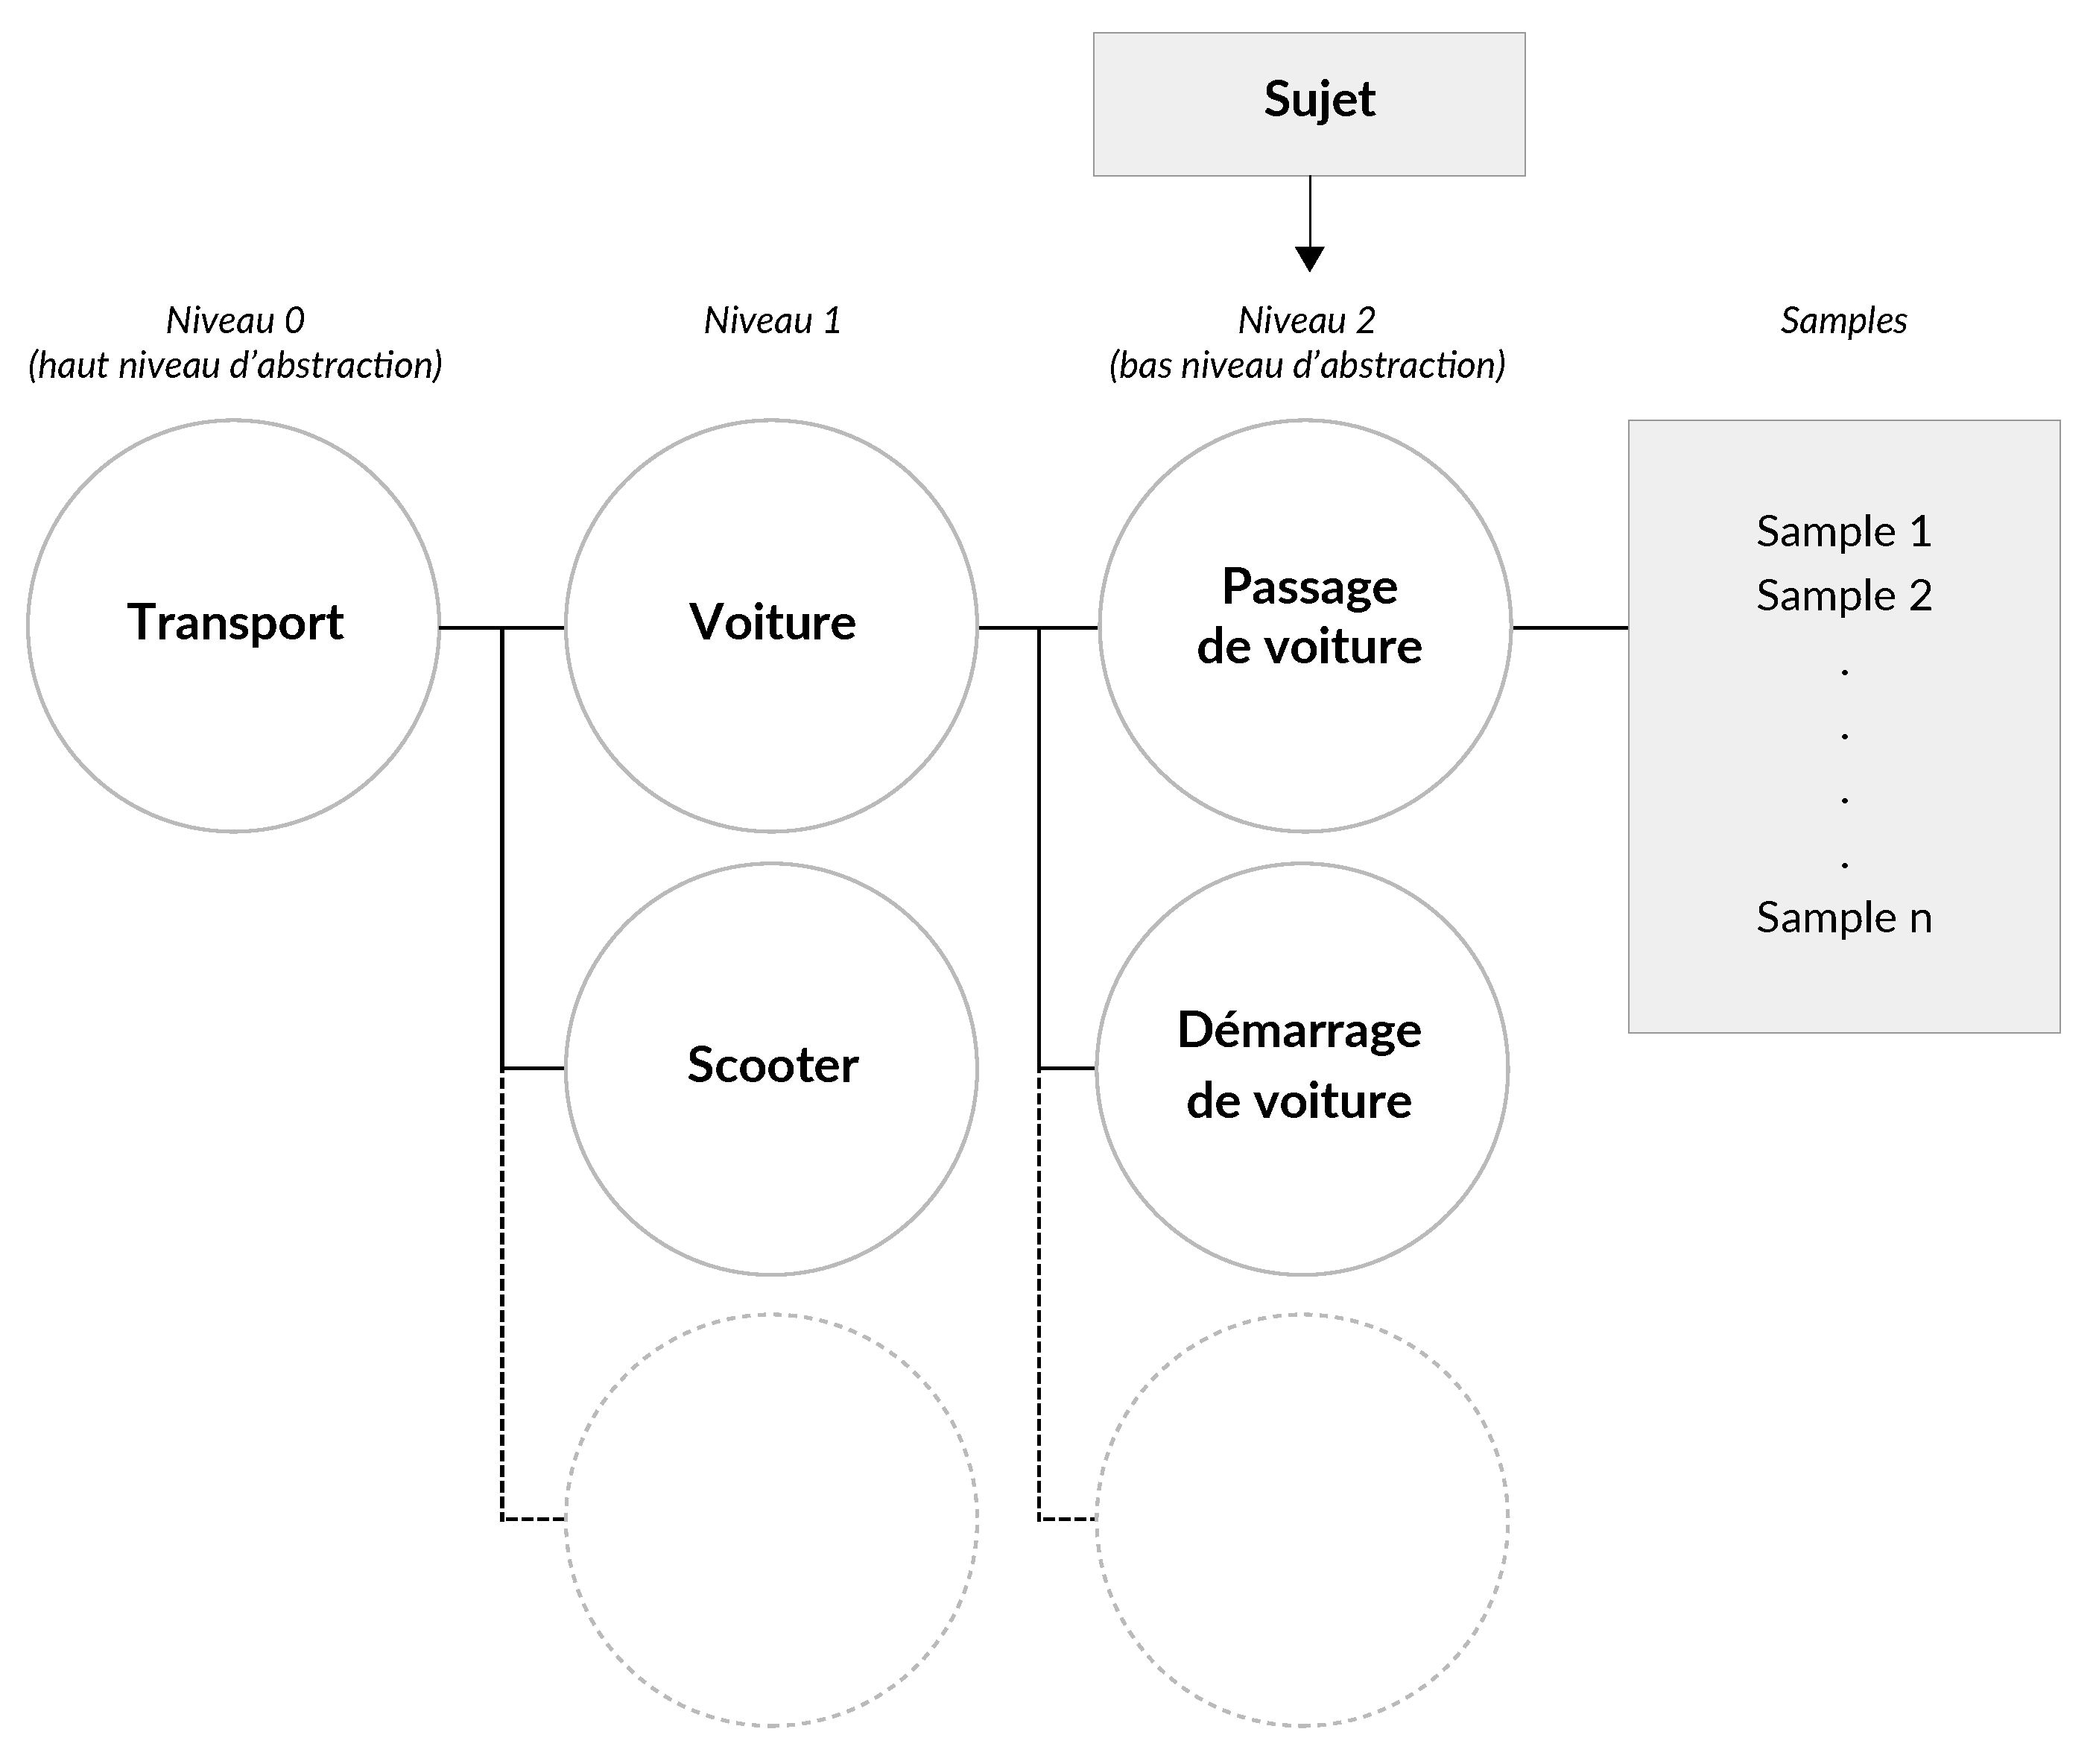
\includegraphics[width=.8\linewidth]{gfx/ch_4/3}
       \caption{Hierachical organisation of the isolated sounds used ofr the simulation.}\label{fig:orgDb}
\end{figure}

%Nous nommons sample, un enregistrement d'un son isolé, événement ou texture. Chaque classe est alors comprise comme une collection de samples jugés perceptivement équivalents.

We term sample, a recording of an isolated sound, be it an event or a texture. Each sound class is implemented as a collection of samples percieved equivalently.

%Les classes de sons sont organisées suivant une structure hiérarchique (\cf~Figure~\ref{fig:orgDb}). Cette structure hiérarchique est largement inspirée de l'axe vertical de l'organisation catégorielle proposée par E. Rosch \cite{rosch1978cognition}, qui dresse une taxonomie des classes ou catégories \ie~plus le niveau d'abstraction de la classe est faible, plus la description de la classe est précise, et plus les sources sonores incluses dans cette classe sont semblables. Si le niveau d'abstraction d'une classe est tel que cette dernière possède des sous-classes, alors sa collection de samples est la somme des collections respectives de chacune des sous-classes.

The sound classes are organized hierachically (\cf~Figure~\ref{fig:orgDb}) according to a structure close to the one of the vertical axis of the categorical organization proposed by E. Rosch \cite{rosch1978cognition}. In this taxonomy, the lower the level of abstraction, the more precise the description of the class and the more perceptually similar the sound sources. For class with high level of abstraction with sub classes, its collection of samples is the union of the collections of the sub classes.

%Nous établissons deux taxonomies, une pour les événements, une autre pour les textures (\cf~Annexe~\ref{app:taxonomie}). Pour les événements, nous considérons quatre niveaux d'abstraction allant des classes les plus générales (niveau d'abstraction 0), aux classes les plus spécifiques (niveau d'abstraction 3). Pour les textures, nous ne considérons que trois niveaux d'abstraction. Notons que la taxonomie des événements est proche de celle de \cite{Salamon14}, introduite postérieurement à notre étude.

Accounting for the perceptual matters detailed previously, two taxonomies are built, one for event sounds and one for texture sounds. Four levels of abstraction are considered from the more generic one (level 0), to the more specific classe (level 3), leading to a taxonomy close to the one used in \cite{Salamon14}. Only three levels of abstraction are considered for the texture sounds.

\subsubsection*{Sound samples collection}

%Sur la base des taxonomies précédemment établies, 483 sons isolés ont été collectés, dont 381 événements, et 102 textures. Parmi ces samples, 332 ont été enregistrés, et 151 proviennent de différentes banques de sons (\emph{SoundIdeas}\footnote{\emph{SoundIdeas}: \url{www.sound-ideas.com}} et \emph{Universal SoundBank}\footnote{\emph{Universal SoundBank}: \url{www.universal-soundbank.com}}).

483 isolated sounds are collected and organized with the two above discussed typologies, 381 events and 102 textures. Among those samples, 332 have been recorded and 151 have been taken from two sound libraries: \emph{SoundIdeas}\footnote{\emph{SoundIdeas}: \url{www.sound-ideas.com}} and \emph{Universal SoundBank}\footnote{\emph{Universal SoundBank}: \url{www.universal-soundbank.com}}.

%Tous les enregistrements ont été effectués à l’aide d'un micro canon \emph{AT8035}\footnote{\emph{Micro canon AT8035}: \url{eu.audio-technica.com}} relié à un enregistreur \emph{ZOOM H4n}\footnote{\emph{ZOOM H4n} : \url{www.zoom.co.jp/english/products/h4n}}. L’utilisation du micro canon nous permet d’isoler les événements sonores du bruit de fond urbain. Pour les textures, il nous permet d’éviter les événements sonores proches du preneur de son. Nous pouvons ainsi pointer des "zones sonores", en nous tenant à une certaine distance de ces dernières, afin de capter uniquement le bruit de fond émanant de la zone ciblée.

Orignal sounds have been recorded using a shotgun microphone \emph{AT8035}\footnote{\emph{Micro canon AT8035}: \url{eu.audio-technica.com}} relié à un enregistreur \emph{ZOOM H4n}\footnote{\emph{ZOOM H4n} : \url{www.zoom.co.jp/english/products/h4n}}. The use of such a microphone allowed us to isolate as much as possible sound events of interest from the urban background. Conversely, it allowed us to avoid dominant sound sources while recording texture sounds by pointing the microphone to distant eareas with no dominant sound sources.

%Tous les sons ont été normalisés au même niveau $RMS$ de $-12$ $dB$ (FS), \ie. relativement à un niveau pleine échelle (\emph{relative to Full Scale}). Dans notre cas, ce niveau pleine échelle est de 1 Volt.

All samples are normalised to the same $RMS$ level of $-12$ $dB$ FS, \ie. relative to Full Scale. In our case, the full scale level is of 1 Volt.

\subsection{Parameters}
\label{sec:simscene_parametre}

%Par choix de conception, l'outil de simulation ne permet pas d’interagir avec un sample en particulier, mais toujours avec une piste, \ie~une séquence de samples. Plusieurs paramètres permettent au sujet de contrôler la structure de chaque piste.

By design, the simulation tool do not allow the user to interect and control a specific sample. Interaction is done at the track level, a track being a sequence of samples. Several paramters are available to the subject to control the track:

% \begin{itemize}
% \item \emph{niveau sonore} ($dB$): pour chaque sample, les niveaux sont tirés aléatoirement à partir d'une distribution normale, paramétrée par le sujet en termes de moyenne et de variance;
% \item \emph{espacement inter-onset} (seconde): (piste d'événements seulement) comme pour les niveaux, les espacements sont tirés aléatoirement à partir d'une distribution normale, paramétrée par le sujet en terme de moyenne et de variance;
% \item \emph{début et fin} (seconde): le sujet fixe le début et la fin de chaque piste.
% \end{itemize}

\begin{itemize}
\item \emph{level} ($dB$): the levels are  randomly sampled according to a normal distribution parametrized by the subject in terms of mean value and variance;
\item \emph{inter-onset spacing} (second): for the event's track only, the spacings arerandomly sampled according to a normal distribution parametrized by the subject in terms of mean value and variance;
\item \emph{start and end time} (second): the subject set the first and last occurence of a sample of the selected class.
\end{itemize}

%Afin de faciliter la simulation, deux paramètres supplémentaires sont proposés:

To ease the simulation, two parameters are also proposed:

% \begin{itemize}
% \item \emph{fondu par événement} (seconde): (piste d'événements seulement) le sujet fixe une durée de fondu (entrée et sortie) appliquée à chaque sample;
% \item \emph{fondu global} (seconde): le sujet fixe les durées de fondus pour l'entrée et la sortie de la piste. Ces fondus s'appliquent ainsi à l'ensemble des samples de la piste.
% \end{itemize}

\begin{itemize}
\item \emph{event's fades} (seconds): for the event's track only, the subject can set a fade in / fade out duration applied to each samples;
\item \emph{global fades} (seconds): the subject set the duration of the fade in /fade out at the beginning and the end of the track.
\end{itemize}

%Deux de ces paramètres ne s’appliquent que pour les pistes d'événements (\emph{fondu par événement}  et \emph{espacement inter-onset}), les samples des textures étant séquencés sans espacement.

The samples of texture are sequenced without time spacing, therefore the parameters \emph{event's fade} and \emph{inter-onset spacing} are not available ofr this kind of track.

\subsection{Selection interface}
\label{sec:simscene_ssf}

%La grande majorité des outils permettant de parcourir une banque de données propose une recherche textuelle sur la base de mots-clé. Dans le cadre d'une expérience sensorielle visant à objectiver la représentation interne du sujet, cette approche est problématique.

%En effet la description verbale du son, si elle est accessible au sujet, peut potentiellement influencer sa sélection. Dans les faits, pour construire une scène environnementale «~calme~», le sujet sélectionne a priori les sons référencés sous le vocable \emph{parc}.

Most of browsing tools are based on keyword indexing. For sensory experiment studying the objectivation of the mental representation of the subject, this mean is problematic as the availability of a verbal description of the sound can influence the choice of the subject. Indeed, the subject will select \textit{a priori} sound referenced belonging to \emph{park} to build a \emph{calm} soundscape.

%Pour limiter l’influence de l’interface sur le sujet, il nous paraît nécessaire de libérer sa recherche de toute information textuelle. Nous proposons à l'utilisateur une interface graphique lui permettant d’explorer la banque de sons exclusivement à partir de l’écoute.

Therefore, the selection interface is text free and composed of spatially organized circles on a two dimensional plane.

%La figure~\ref{fig:ssf} présente l'interface pour la banque de données d'événements sonores. Visuellement, les classes du dernier palier (niveaux d'abstraction 3 pour les événements, 2 pour les textures) sont représentées par des cercles, et positionnées sur un plan. La disposition des cercles dans l'espace dépend de l’organisation hiérarchique de la base de données: les sous-classes appartenant à une même classe sont proches les unes des autres, et ainsi de suite jusqu'à atteindre les classes du dernier palier, les seules auxquelles le sujet peut accéder, des classes qui ne possèdent pas de sous-classes, et sont directement liées à une collection de samples.

The Figure~\ref{fig:ssf} shows the interface used for the selection of events. The classes of the higher level of abstraction are plotted with circles. The spatial location of the circles is chosen according to the hierarchical organization of the sound database: sub-classes belonging to the same class are close to each others, and so on until the user reaches the lower level classes displayed in grey which are directly linked to a collection of samples.

%Chaque classe du dernier palier possède un son prototype. Ces sons ont été choisis par les expérimentateurs. Lorsqu’on clique sur un cercle, le prototype associé à la classe est joué. Le sujet parcourt la banque de sons en cliquant sur les cercles. Cette interface a fait l'objet d'une étude approfondie dont les résultats sont publiés dans \cite{lafay2016JAES}.

Each of those classes have a representative sound chosen arbitrarily by the authors in order to provide the same sound each time the user clicks on the circle. The subject can browse the database by listening to those prototype sound. The efficiency of this interface compared to several others designs have been evaluated and the outcomes are discussed in \cite{lafay2016JAES}.

\begin{figure}[t]
        \myfloatalign
        \subfloat[]
        {\includegraphics[width=.8\columnwidth]{gfx/ch_4/SSF}\label{fig:ssf}} \par
        \subfloat[]
        {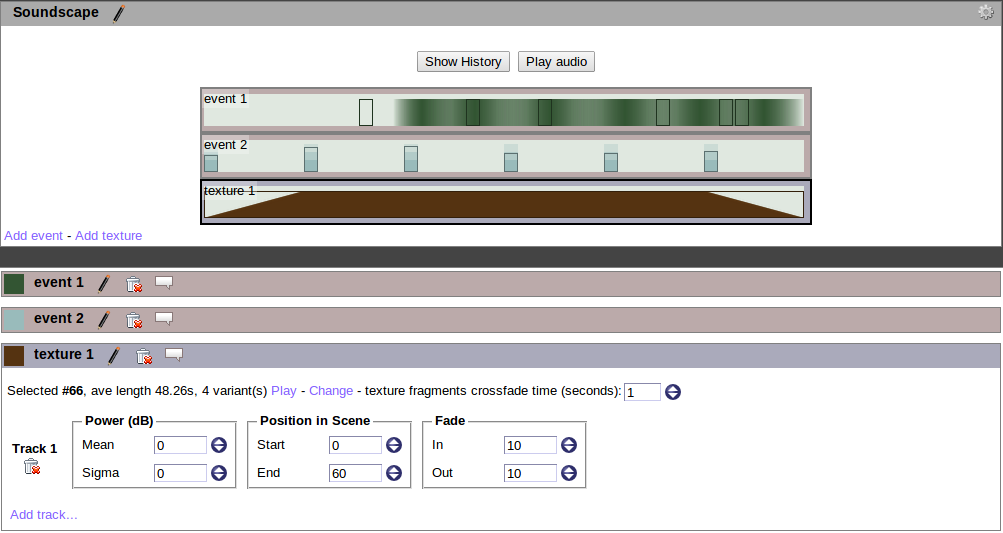
\includegraphics[width=\columnwidth]{gfx/ch_4/simscene}\label{fig:simscene}}
       \caption{Visual interfaces for the selection of sound classes (a) and their sequencing (b) of the \emph{Simscene} tool.}
\end{figure}

\subsection{Simulation interface}

%L'interface de simulation propose un rendu graphique schématisé de la scène en cours de création (\cf~Figure~\ref{fig:simscene}). La piste est représentée par une bande possédant un axe temporel. Sur cette bande, chaque sample est représenté par un rectangle. L'espacement entre les rectangles est fonction de l'espacement entre les samples. De même, la hauteur des rectangles est proportionnelle au niveau sonore des samples. Dans le cas d'une piste de texture, un unique rectangle apparaît sur toute la longueur de la piste, un son de texture ne pouvant être entrecoupé de silences. Les caractéristiques des rectangles évoluent en fonction des changements de paramètres de la piste. L'utilisateur a la possibilité, à tout moment, d'écouter la scène simulée.

As shown on Figure~\ref{fig:simscene}, the simulation interface displays a schematic of the scene under creation. Each track is represented as an horizontal band with a temporal axis. Each sample of this track is displayed by a rectangle whose height is proportional to the amplitude of the sample. For event's tracks, the horizontal spacing between those rectangles is a function of the time delay between their onsets. For tracks of texture, a unique rectangle is displayed as this kind of sounds do not allow spacing with silence. As actual amplitude and spacing values are drawn from random variables, each time the subject changes the value of a parameter, the location and height of the rectangles are updated to reflect the changes in the sequencing of the samples. The subject can listen to the resulting sound scene.

%La scène sonore est ainsi vue comme une somme de sources sonores, ou, si l'on admet la distinction opérée entre événements et textures sonores, «~un squelette d'événements sur un lit de textures~» \cite{nelken2013ear}. Cet outil de simulation est présenté en détail dans \cite{rossignol2015simscene}.

As such, the underlying model of the scene is a sum of sound sources, more precisely a "skeleton of events on a bed of textures" \cite{nelken2013ear}. Further details about the simulation interface can be found in \cite{rossignol2015simscene}.

\section{Experiment 2: modification of the semantic content}
\label{sec:xp3}

\subsection{Objective}

%L'expérience précédente a montré que, parmi les classes de sons peuplant le monde sonore, celles regroupant les marqueurs sont caractéristiques de certains types d'environnement. Ces marqueurs sonores semblent avoir un impact particulier sur la perception de leurs environnements. C'est ce dernier point qui est étudié dans cette expérience.

The previous experiment demonstrated that, among the classes of sounds occuring in urban soundscapes, those with markers are specific of some of environments. Those sound markers seem to have a great impact on perception. This impact is studied in more detail using an added benefit of the simulation paradigm proposed in this paper, the ability to manipulate and modify the generated scenes.

%Afin de vérifier que l'agrément des scènes idéales et non-idéales dépend de la présence des marqueurs, les scènes sonores précédemment simulées sont régénérées, sans les classes de marqueurs. Pour les i-scènes, les i-marqueurs sont retirés. Pour les ni-scènes, les ni-marqueurs. Une épreuve d'évaluation de l'agrément, dont le protocole se rapproche de celui de l'expérience 1.b, est alors conduite.

In order to verify that the pleasantness of the ideal and non ideal scenes if affected by the sound markers, the audio waveforms of the simulated scenes are regenerated without considering the classes identified as markers. For the i-scenes, the i-markers are removed. For the ni-scenes, the ni-markers are removed. A perceptive test evaluating the pleasantness is conducted with a protocol close to the one considered in experiment 1.b.

%L'objectif est de vérifier si l'absence des marqueurs a un impact sur l'agrément perçu. Deux hypothèses sont formulées:

Thus the objective of this experiment is to study if the removal of the previously identified markers have an impact on the percieved pleasantness. Two hypothesis are formulated:

%\begin{itemize}
% \item \emph{pour les ni-scènes} nous faisons l'hypothèse que l'absence des ni-marqueurs va \textbf{augmenter} la valeur de l'agrément perçu;
% \item \emph{pour les i-scènes} nous faisons l'hypothèse que l'absence des i-marqueurs va \textbf{diminuer} la valeur de l'agrément perçu.
% \end{itemize}

\begin{itemize}
\item \emph{for the ni-scenes} we hypothesize that the absence of ni-markers will \textbf{increase} the pleasantness score;
\item \emph{for the i-scenes} we hypothesize that the absence of the i-markers will \textbf{decrease} the pleasantness score.
\end{itemize}

%Si la première hypothèse est intuitive, la deuxième l'est moins. En effet, il n’apparaît pas évident que la suppression des i-marqueurs, bien que s'agissant de sons positivement connotés, diminue la qualité globale d'un environnement. Cette suppression aura, de surcroît, pour effet de diminuer le niveau sonore global de la scène.

If the first hypothesis is rather intuitive, the second is less. Indeed, it is not obvious that the removal of the i-markers, though perceptively connoted, decreases the global quality of a soundscape. This removal also decreases the global level of the scene.

%Néanmoins, comme nous l'avons vu, le niveau global n'est qu'un indicateur partiel de l'agrément pour les environnements sonores idéaux. Qui plus est, cet indicateur, lorsque qu'il décrit le niveau des i-marqueurs, impacte de manière positive la qualité de la scène. L'hypothèse mérite donc d'être vérifiée.

Though, as discussed before, the global amplitude level can only be considered as a partial indicator of pleasantness of the ideal soundscapes. Furthermore, the level of i-markers positively impact the pleasantness. For those reasons, the validation of the second hypothesis is of high interest.

\subsection{Planification of experiment 2}

\subsubsection*{Stimuli}

%La banque de données de stimuli compte 144 séquences de 30 secondes. Ces 144 séquences comprennent:
% \begin{itemize}
% \item \emph{72 am-scenes}: les 72 scènes précédemment simulées, avec les classes de marqueurs (am). Nous notons i/am-scènes, les 36 scènes idéales avec marqueurs, et ni/am-scènes les 36 scènes non-idéales avec marqueurs;
% \item \emph{72 sm-scènes}: les 72 scènes précédemment simulées, régénérées sans les classes de marqueurs (sm). Nous notons i/sm-scènes, les 36 scènes idéales sans marqueurs, et ni/sm-scènes les 36 scènes non-idéales sans marqueurs.
% \end{itemize}

There are 144 stimuli of 30 seconds durations. More precisely:

\begin{itemize}
\item \emph{72 km-scenes}: the 72 scenes originally simulated by the subject of experiment 1.a where the sound classes identified as markers are kept. The 36 ideal scenes with markers are noted i/km-scenes, and the 36 non ideal scenes with markers are noted ni/km-scenes.
\item \emph{72 rm-scènes}:  72 scenes where the sound classes identified as markers are removed. The 36 ideal scenes without markers are noted i/rm-scenes, and the 36 non ideal scenes without markers are noted ni/rm-scenes.
\end{itemize}


%Nonobstant l'absence des marqueurs, les am- et sm-scènes sont en tout point semblables.

Notwithstanding the presence or absence of markers, the km-scenes and rm-scenes are exactely the same.

%Nombre de am-scènes sont composées, en majorité, de samples de marqueurs. Afin de ne pas dénaturer abusivement ces scènes, en créant notamment des temps de «~vide~», \ie~ne comprenant aucun sample, nous ne supprimons que les marqueurs des classes d'événements du premier niveau d'abstraction (\cf~Tableau~\ref{tab:markers}). Ces classes sont:

In order to create km-scenes with still some sound diversity and no long duration absence of sound activity within the scene, only the sound classes of events of the first level of abstraction are removed, see Table~\ref{tab:markers}. Those classes are:

% \begin{itemize}
% \item \emph{cloche}, \emph{sonnette de vélo}, \emph{animaux} pour les i/sm-scènes;
% \item \emph{sirène}, \emph{klaxon} pour les ni/sm-scènes.
% \end{itemize}

\begin{itemize}
\item \emph{Church bell}, \emph{bicycle bell}, \emph{animals} pour les i/sm-scènes;
\item \emph{siren}, \emph{car horn} pour les ni/sm-scènes.
\end{itemize}

%Il est important de noter ici que tous les i- et ni-marqueurs ne sont donc pas supprimés dans les sm-scènes.

Thus, only a fraction of the i-markers and ni-markers are removed in the rm-scenes.

\subsubsection*{Experiment}

Les sujets évaluent les 144 scènes. L'évaluation s'effectue sur une échelle sémantique bipolaire de 11 points allant de -5 (non-idéale/très désagréable) à +5 (idéale/très agréable). Avant de noter une scène, les sujets doivent obligatoirement en écouter les 20 premières secondes. Après la notation, ils sont libres de passer à la scène suivante.

Pour chaque sujet, les scènes sont présentées dans un ordre aléatoire. Les 10 premières scènes permettent au sujet de calibrer ses notes. Elles sont obligatoirement composées de 5 i/am-scènes et de 5 ni/am-scènes. Ces 10 premières scènes sont rejouées à la fin de l'expérience, et seules les notes données à la deuxième occurrence sont prises en compte.

L'expérience est prévue pour durer 1 heure. Les sujets ne connaissent pas la nature des scènes.

\subsubsection*{Experimental protocol}

%Tous les sujets passent l'expérience sur des machines identiques. L'audio est diffusé en monophonie, par le biais de casques audio semi-ouverts \emph{Beyer-Dynamic DT 990 Pro}. Toutes les scènes sonores ont été re-simulées sur la base des partitions obtenues lors de l'expérience de simulation. Le niveau sonore de sortie est identique pour tous les sujets.

All the subjects perform the test on the same type of computers . Thy listen to the stimuli with semi-open \emph{Beyer-Dynamic DT 990 Pro} headphones. The sound level is the same for all subjects.

%Tous les sujets réalisent l'expérience simultanément, dans un environnement calme. Ils n'ont pas le droit de s'adresser la parole pendant l'expérience.

All the subjects perform the test at the same time, in a quiet environment. They are not allowed to talk to each other during the experiment.

%Un expérimentateur est présent durant la totalité de l'expérience, afin de contrôler le bon déroulement de cette dernière, et de répondre aux éventuelles questions des sujets.

A supervisor is available during the whole duration of the experiment to ensure a smooth running of the latter and answer any questions the subjects may have.

\subsubsection*{Participants}

%12 sujets (4 femmes) participent à l'expérience. Aucun d'entre eux n'a réalisé l'expérience de simulation, ni la première expérience d'évaluation. Les sujets sont âgés de 22 à 61 ans (moyenne: 29.5, écart-type: 14). Tous les sujets sont Nantais, et vivent dans cette ville depuis deux ans ou plus.Tous les sujets ont réalisé l'expérience avec succès.

12 subjects (4 womens) perform the test. None of them have performed experiments 1.a and 1.b. The subjects are 22 to 61 years old (average: 29.5, standard deviation: 14). All the subjects live in Nantes, France, for at least two years. All the subjects performed the test succesfully.

\subsection{Data and analysis method}

%Les données analysées sont les mêmes que pour la première expérience. Nous invitons le lecteur à se référer à la section~\ref{sec:xp1_dataAna} pour plus de détails.

The type of data analysed in this experiment have been considered for experiment 1.a, see Section~\ref{sec:xp1_dataAna} for details.

%Il s'agit ici de vérifier que la suppression des i- et ni-marqueurs impacte l'agrément perçu. Pour ce faire, nous utilisons l'analyse de variance. Nous considérons, comme variable dépendante, $\mathcal{A}_{sujet}$, et, comme variables indépendantes, le type d'environnement (i/ni), et la présence/absence de marqueurs (am/sm). Chaque sujet devant évaluer la totalité des stimuli, une ANOVA à mesures répétées à deux facteurs est utilisée afin vérifier s'il existe des différences significatives d'agrément perçu. Les deux variables indépendantes sont considérées comme des facteurs intra-sujet (\emph{within-subject}. Les facteurs n'étant composés que de deux niveaux chacun (type: i/ni; marqueur: am/sm), l'hypothèse de sphéricité n'a pas besoin d'être vérifiée. Les analyses \emph{post hoc} sont conduites en appliquant la procédure de Tukey-Kramer.

The aim here is to validate the hypothesis that the removal of i-markers and ni-markers have an impact on the perceived pleasantness. To do so, we perform a variance analysis. We consider $\mathcal{A}_{sujet}$ as a dependant variable, and as independant variables, the type of envorinment (i/ni), and the presence/absence of markers (km/rm). As each subject evaluated the whole set of scenes, a two factors repeated measure ANOVA is used in order to verify the hypothesis that there exist a significant difference of percieved pleasantness between km-scenes and rm-scenes. The two independant variables are cosidered as \emph{within-subject} factors. The factors being of only two levels each (type: i/ni; marker: km/rm), the sphericity impothesis does not need to be checked. \emph{Post hoc} analysis are done by following the Tukey-Kramer procedure.

%Tous les tests de significativité sont effectués avec un seuil critique $\alpha=0.05$.

All the significance tests are done using a critical threshold $\alpha=0.05$.

\subsection{Results}

\subsubsection{Outliers detection}

%Considérons $\mathcal{A}_{sujet}$ pour les am-scènes. Il apparaît que les réponses d'un des sujets diffèrent des autres. Ce dernier a évalué positivement près de la moitié des ni/am-scènes (\cf~Annexe~\ref{app:xp2} : sujet 7). Le sujet a donné à 58\% des ni/am-scènes une note supérieure à 0, contre une moyenne de 11\% pour les autres sujets. De plus, le sujet a utilisé l'ambitus maximal (-5 à 5) pour noter à la fois les i/ et ni/am-scènes. Ces faits n'ayant pas été observés pour les autres sujets, que l'on considère les expériences 2 ou 1.b, le sujet 7 est éliminé de l'analyse.

Let us consider $\mathcal{A}_{sujet}$ for the km-scenes. Close inspection that the answers given by one subject strongly differs with the ones of others. This subject evaluated positively close to half of the ni/km-scenes, see Annex~\ref{app:xp2}, subject 7. This subject gave a grade above 0 for 58\% of the ni/km-scenes, contrary to an average of 11\% for the remaining of the subjects.

Furthermore, this subject used the whole scale (from -5 to 5) to grade both the i-scenes and the ni-scenes. Those behaviors strongly differing with the ones of the others subjects be they from this experiment or the previous ones, we decide to discard the subject 7 from the analysis.

\subsubsection{Influence of the markers on perceived pleasantness}

%Dans cette section nous étudions comment les sujets ont perçu les différents types de scènes, nommément: i/am-, ni/am-, i/sm- et ni/sm-scène. L'ANOVA à mesures répétées pratiquée sur $\mathcal{A}_{sujet}$ montre un effet significatif du type d'environnement (i/ni: $F[1,10]=175$, $p<0.01$), de la présence/absence des marqueurs (am/sm: $F[1,10]=7$, $p<0.05$), ainsi que de l'interaction entre les deux facteurs ($F[1,10]=67$, $p<0.01$).

In this section, we study the grades given by the subject while listening to the several types of scenes, namely the i/km-scenes, ni/km-scenes, i/rm-scenes et ni/rm-scenes. The repeated measure ANOVA applied to $\mathcal{A}_{sujet}$ exhibit a significative effect of the type environment (i/ni: $F[1,10]=175$, $p<0.01$), of the presence/abscence of markers (km/rm: $F[1,10]=7$, $p<0.05$), and of the interaction between those two factors ($F[1,10]=67$, $p<0.01$).

%The \emph{post hoc} montre, quant à elle, des différences significatives entre tous les groupes d'observations, notamment entre les i/am- et i/sm-scenes ($p<0.05$) et les ni/am- et ni/sm-scenes ($p<0.01$).

The \emph{post hoc} analysis exhibit significative differences between all the groups of observations, notably between the i/km-scenes ($p<0.05$) and the i/rm-scenes ($p<0.01$).

%Ces résultats indiquent que la suppression des événements a effectivement modifié la perception des scènes par les sujets. Nos deux hypothèses sont ainsi vérifiées:

These results indicate that the removal of the markers did indeed modify the perception of the scenes by the subjects. Our two hypotheses are thus verified:

% \begin{itemize}
% \item la suppression des ni-marqueurs a amélioré les qualités perçues des ni-scènes;
% \item la suppression des i-marqueurs a diminué les qualités perçues des i-scènes.
% \end{itemize}

\begin{itemize}
\item the removal of the ni-markers improved the pleasantness of the ni-scenes;
\item the removal of the i-markers reduced the pleasantness of the i-scenes.
\end{itemize}

%L'interaction significative montre que l'effet du type d'environnement influe sur l'effet de l'absence/présence des marqueurs. En effet la moyenne des écarts entre am- et sm-scènes est plus importante pour les ni-scènes ($1.1$) que pour les i-scènes ($0.5$).

The significative interaction shows that the effect of the type of environment influences the effect of the presence/absence of the markers. Indeed, the average of the differences between km-scenes and rm-scenes is larger for the ni-scenes ($1.1$) than for the i-scenes ($0.5$).

\subsection{Discussion}

%Cette expérience fait apparaître que la présence, dans une scène, des marqueurs relevés à l'expérience 1 impacte bien l'agrément perçu. La suppression des ni-marqueurs a un effet bénéfique sur le ressenti des ni-scènes, tandis que, plus surprenant, la suppression des i-marqueurs dégrade légèrement la qualité des i-scènes. Ce dernier point est d'autant plus marquant que, du fait de la suppression des marqueurs, le niveau des i/am-scènes est supérieur à celui des i/sm-scènes.

This experiment shows that the presence of markers identified during the analysis of experiment 1 does have an impact on the percieved pleasantness. The removal of the ni-markers has a positive effect on the perception of the ni-scenes. Perhaps more surprisingly the removal of the i-markers slightly decreases the perception of the i-scenes. This is even more striking because, due to the removal of the markers, the acoustic pressure level of the i/km-scenes is higher than the one of the i/rm-scenes.

%Les i-marqueurs ont donc bien un effet bénéfique sur la perception d'un environnement. Le fait que leur suppression diminue $\mathcal{A}_{scene}$ montre clairement qu'il est possible d'améliorer la qualité sonore d'un lieu en ajoutant des sons bien acceptés comme \emph{oiseau}. Ces conclusions vont dans le sens de l'approche positive introduite par Schafer \cite{schafer1977tuning}.

So the i-markers do have a positive impact on the perception of an environment. The fact that their removal decreases $\mathcal{A}_{scene}$ clearly shows that it is possible to improve the perceived pleasantnes of a given place by the addition of sounds commonly considered as pleasant such as \emph{brid calls}. Those conclusions are in line with the positive approacj introduced by Schafer in \cite{schafer1977tuning}.

%%%%%%%%%%%%%%%%%%%%%%%%%%%%%%%%%%%%%%%%%%%%%%%%%%%%%%%%%%%%
%%%%%%%%    DISCUSSION AND PERSPECTIVES   %%%%%%%%%%%%%%%%%%
%%%%%%%%%%%%%%%%%%%%%%%%%%%%%%%%%%%%%%%%%%%%%%%%%%%%%%%%%%%%


\section{Outcomes for sounscape perception}

%Les expériences ont montré que la majorité des descripteurs utilisés, qu'ils soient sémantiques ou structurels, permettent de faire la distinction entre une scène idéale et une scène non-idéale.

This series of three experiments showed that most of the descriptors used in this study, be they semantic or compositional, allows us to distinguish between a said ideal scene et a non ideal one.

%Cependant, nous observons que les caractéristiques physiques corrélées à l'agrément diffèrent clairement suivant le type de scènes. Dans le cas des scènes idéales, c'est avant tout l'émergence de marqueurs sonores qui détermine la qualité perçue, alors que dans le cas des scènes non-idéales, c'est le niveau sonore global qui influe sur l'agrément.

That being said, we observe that the physical caracteristics correlated with the perceived pleasantness clearly differ depending on the type of scenes. In the case of ideal scenes, it is above all the emergence of sound markers that determines the perceived quality, whereas in the case of non-ideal scenes, it is the overall sound level that proeminently influences the perceived quality.

%Ces résultats tendent à confirmer que la perception des qualités d'une scène dépend avant tout des sources sonores qui la composent, les caractéristiques structurelles mobilisées dans le processus perceptif semblant varier d'une source à l'autre, et d'un type d'environnement à l'autre. Ce fait montre qu'il est illusoire d'envisager qu'un descripteur physique holistique puisse rendre compte, de manière pertinente, des qualités affectives de tous types d'environnement.

These results tend to confirm that the perception of the qualities of a scene depends above all on the sound sources that compose it, the compostional characteristics taken into accound during the perceptual process appearing to vary from one source to the other, from one type of environment to the other. This fact lead the authors to conclude that there is little hope to find a holistic physical descriptor that can adequately account for the affective qualities of all types of sound environment.

%Cet état de fait peut potentiellement influer sur les stratégies à adopter pour améliorer la qualité de l’environnement sonore:

Those results may have an impact on the relevant strategies to adopt while trying to improve the quality of a sound environment:

% \begin{itemize}
% \item dans le cadre de scènes non-idéales, il s'agit de diminuer le niveau sonore, soit de manière globale, soit en agissant sur certaines sources (\emph{sirène}, \emph{klaxon});
% \item dans le cadre de scènes idéales, il s'agit 1) d'identifier les sons agréables, \ie~les marqueurs sonores, 2) de baisser le niveau des autres sons, 3) voire, en restant dans la limite du raisonnable, d'augmenter le niveau des marqueurs par rapport aux autres sons.
% \end{itemize}

\begin{itemize}
\item in the case of non ideal scenes, one such focus on reducing the acoustic pressure level, wether globally, or by discarding specific sources such as \emph{sirens} or \emph{car horns}
\item in the case of ideal scenes, one should first idenity which sources are pleasant to the targeted community, second lower the volume of the other sound sources, and, if possible, raise the contribution or add positive sound markers.
\end{itemize}

%Ces travaux nous permettent enfin de conjecturer quant à la nature des représentations mentales des concepts «~environnement sonore urbain agréable~» (EA) et «~environnement sonore urbain désagréable~» (ED).

Finally, these works allow us to conjecture as to the nature of the mental representations of the concepts "pleasant urban sound environment" (EA) and "unpleasant urban sound environment" (ED).

%Premièrement, le fait que les informations sémantiques (sources sonores présentes) et structurelles soient différentes pour les scènes idéales et non-idéales nous porte à croire que ces deux types d'informations caractérisent les concepts EA et ED.

First, the fact that the semantic information (in terms of which sound sources are present) and compositional information are different for ideal and non-ideal scenes leads us to believe that these two types of information characterize the EA and ED concepts.

%Deuxièmement, le fait que la suppression des marqueurs sonores modifie l'agrément perçu nous porte à croire que le concept abstrait lié à l'agrément (\eg. scène agréable) dépend de l'activation d'un réseau de concepts concrets liés aux sources (dans notre cas \emph{oiseau}, \emph{cloche} et \emph{sonnette vélo}).

Secondly, the fact that the removal of sound markers modifies the perceived pleasantness leads us to believe that the abstract concept related to pleasantness depends on the activation of a network of concrete concepts strongly linked to the sources which are in the case of this study: \emph{bird}, \emph{church bell} and \emph{bicycle bell}).

%Troisièmement, le fait que les descripteurs structurels corrélés à l'agrément diffèrent en fonction du type de scènes nous porte à croire que les caractéristiques structurelles permettant de distinguer deux instances d'un même concept abstrait lié à l'agrément ne sont pas les mêmes pour EA et ED.

Third, the fact that the compositional descriptors correlated with the percieved pleasantness change according to the type of scenes leads us to believe that the compositional characteristics allowing to distinguish two instances of the same abstract concept linked to the pleasantness are not the same for EA and ED.

\section{Conclusion}

%Au terme de notre étude, nous pensons que la simulation est un outil dont le développement pourrait permettre aux décideurs en matière d'urbanisme d'interroger toute une communauté sur ses représentations propres des environnements sonores auxquels elle est exposée, et, pourquoi pas, sur les représentations des environnements sonores auxquels elle voudrait être exposée.

In the opiion of the authors, the study described in this paper demonstrate strongly the usefulness of considering simulation tools such as \emph{simScene} in order to scientifically question  the perception of soundscapes. We also believe that its wider usage could enable urban planning decision-makers to question an entire community about its own representations of the sound environment to which it is exposed, and about the representations of the sound environments to which it would like to be exposed.

Dans la continuité des travaux réalisés, il conviendrait de multiplier les expériences de simulation, en faisant varier les qualités affectives (calme, confortable, gênante, \etc), mais aussi en spécifiant des lieux particuliers (parc, place, rue, \etc), afin d'élaborer des corpus entiers de scènes cognitivement renseignées de paysages sonores.

Il serait par ailleurs intéressant d'utiliser la simulation afin d'étudier plus avant les effets provoqués par la modification volontaire d'une caractéristique d'une scène, comme lors de la suppression des marqueurs sonores pratiquée dans l'expérience 2.

Une des pistes privilégiée dans ce cadre serait d'étudier l'impact de l'ajout de marqueurs sonores positivement appréciés à une scène non idéal pour étudier l'hypothèse que ce type d'ajout améliorerait la qualité perçue de la scène.

Enfin, l'on pourrait encore étudier l'influence des contextes socio-culturels sur la perception. Dans les faits, si le son de cloche est le plus souvent un marqueur d'environnement de qualité pour un occidental, cela ne se vérifie pas nécessairement auprès de sujets de culture orientale, moyen-orientale ou autre.

Outre les possibilités déjà évoquées, le protocole de simulation présenté ici ainsi que son implémentation apporte encore dans ce cas deux avantages:

\begin{itemize}
\item le simulateur peut être déployé à large échelle via internet du fait de l'architecture logicielle choisie pour son développement;
\item les scènes simulées peuvent être analysées sans avoir à tenir compte des différentes langues maternelles des sujets, la nature sémantique des classes de sons utilisées étant connue \emph{a priori} par l'expérimentateur et sans avoir besoin d'analyser la scène sonore pour idientifier les sources, leurs présences dans la scène étant directement exploitable.
\end{itemize}

%Bien évidemment, ces approches nécessitent d'accroître la taille des banques de sons isolés disponibles, un effort conséquent, mais nécessaire, qui contribuera grandement aux nombreux domaines de recherche ayant trait aux scènes sonores.

\nm{a ce propos, il n'est pas fait mention des sons manquants pour les participants (cf. protocole expe de 1a);
ne faudrait -il pas en dire 2 mots ce qui alimenterait aussi la discussion sur la dependance de la qualite (et l'efficacite) de la simulation a  la constitution de la base de donnees de textures et d'evenemetns ?}

\section*{\normalsize Acknowledgements}
\setlength{\parindent}{0.7cm}
Research project partly funded by ANR-11-JS03-005-01. The authors would like to thank the students of the Ecole Centrale de Nantes for their willing participation.


%%%%%%%%%%%%%%%%%%%%%%%%%%%%%%%%%%%%%%%%%%%%%%%%%%%%%%%%%%%%
%%%%%%%%%%%%%%%%    Bibliography    %%%%%%%%%%%%%%%%%%%%%%%%
%%%%%%%%%%%%%%%%%%%%%%%%%%%%%%%%%%%%%%%%%%%%%%%%%%%%%%%%%%%%

\References{}{Bibliography}{actalit}

%%%%%%%%%%%%%%%%%%%%%%%%%%%%%%%%%%%%%%%%%%%%%%%%%%%%%%%%%%%%
%%%%%%%%%%%%%%%%%%%    APPENDICES   %%%%%%%%%%%%%%%%%%%%%%%%
%%%%%%%%%%%%%%%%%%%%%%%%%%%%%%%%%%%%%%%%%%%%%%%%%%%%%%%%%%%%

\onecolumn

\appendix
\section{Taxonomies des classes de sons}
\label{app:taxonomie}

\begin{figure}[h]
        \myfloatalign
        \subfloat[]
        {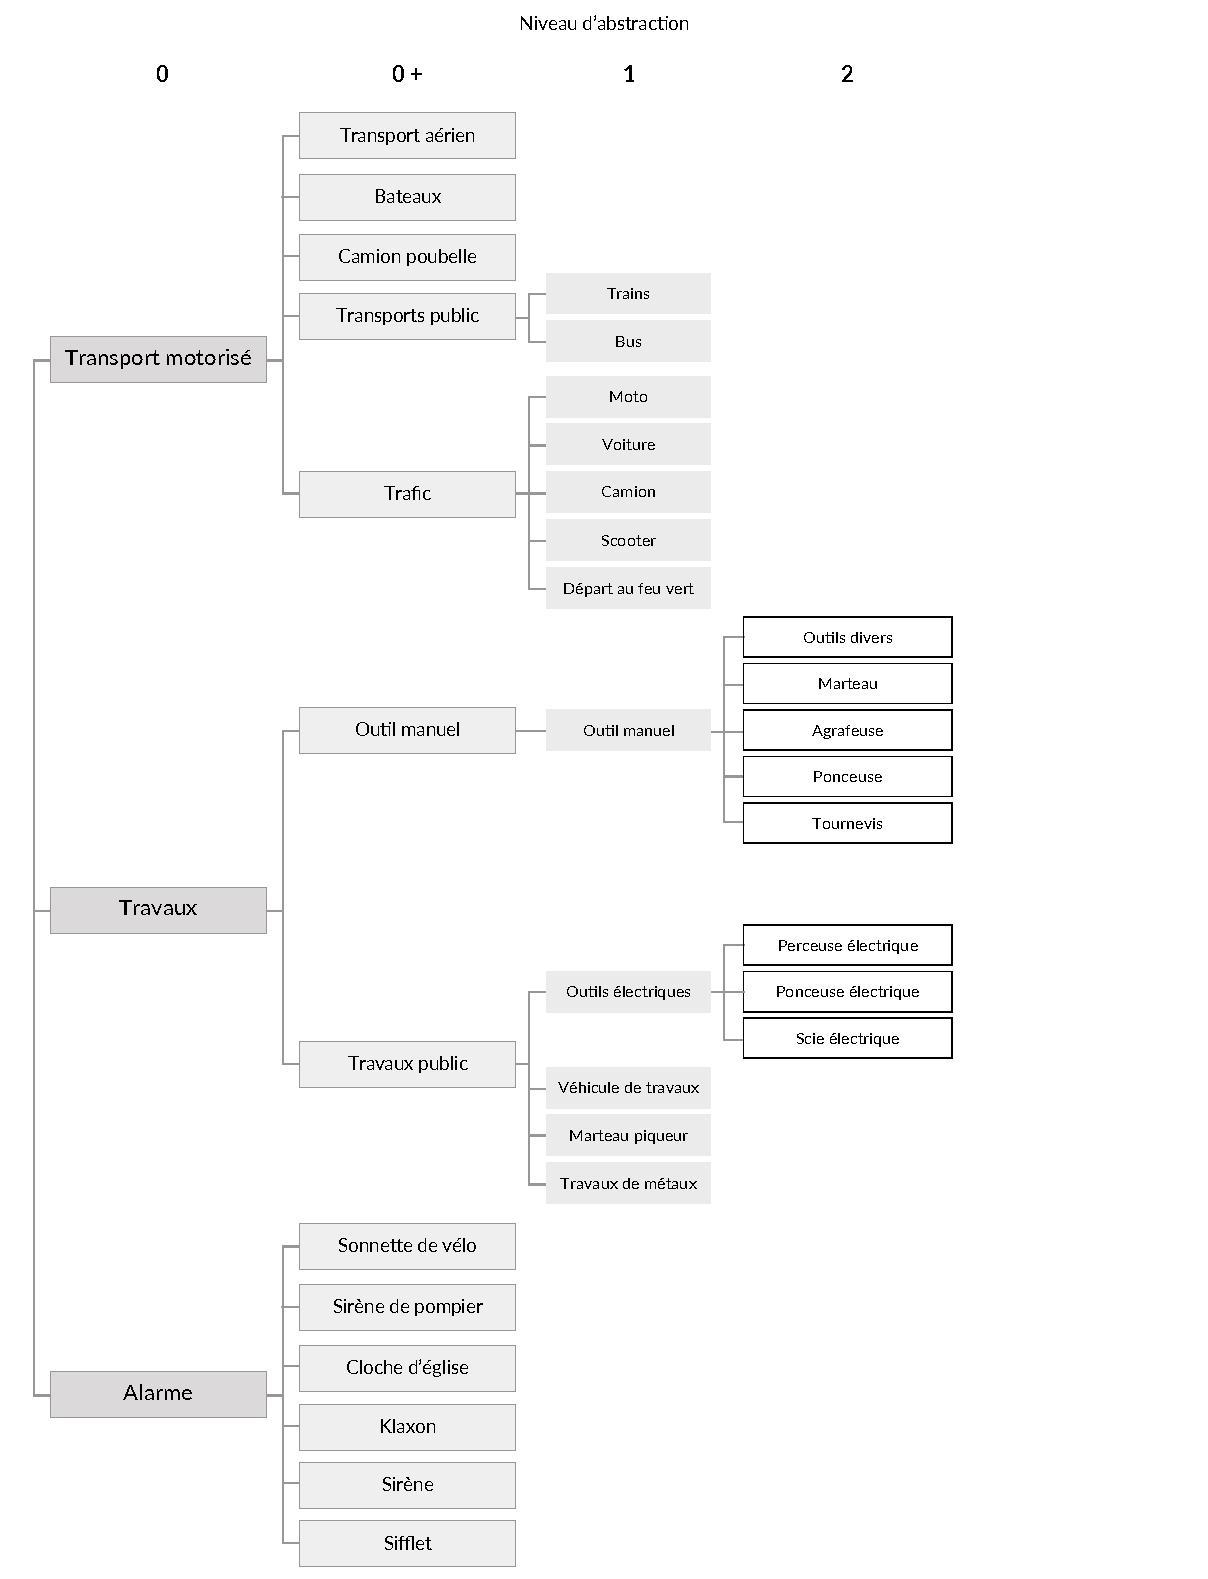
\includegraphics[width=.5\columnwidth]{gfx/ch_5/event_1}\label{fig:taxonomieEventa}}
        \subfloat[]
        {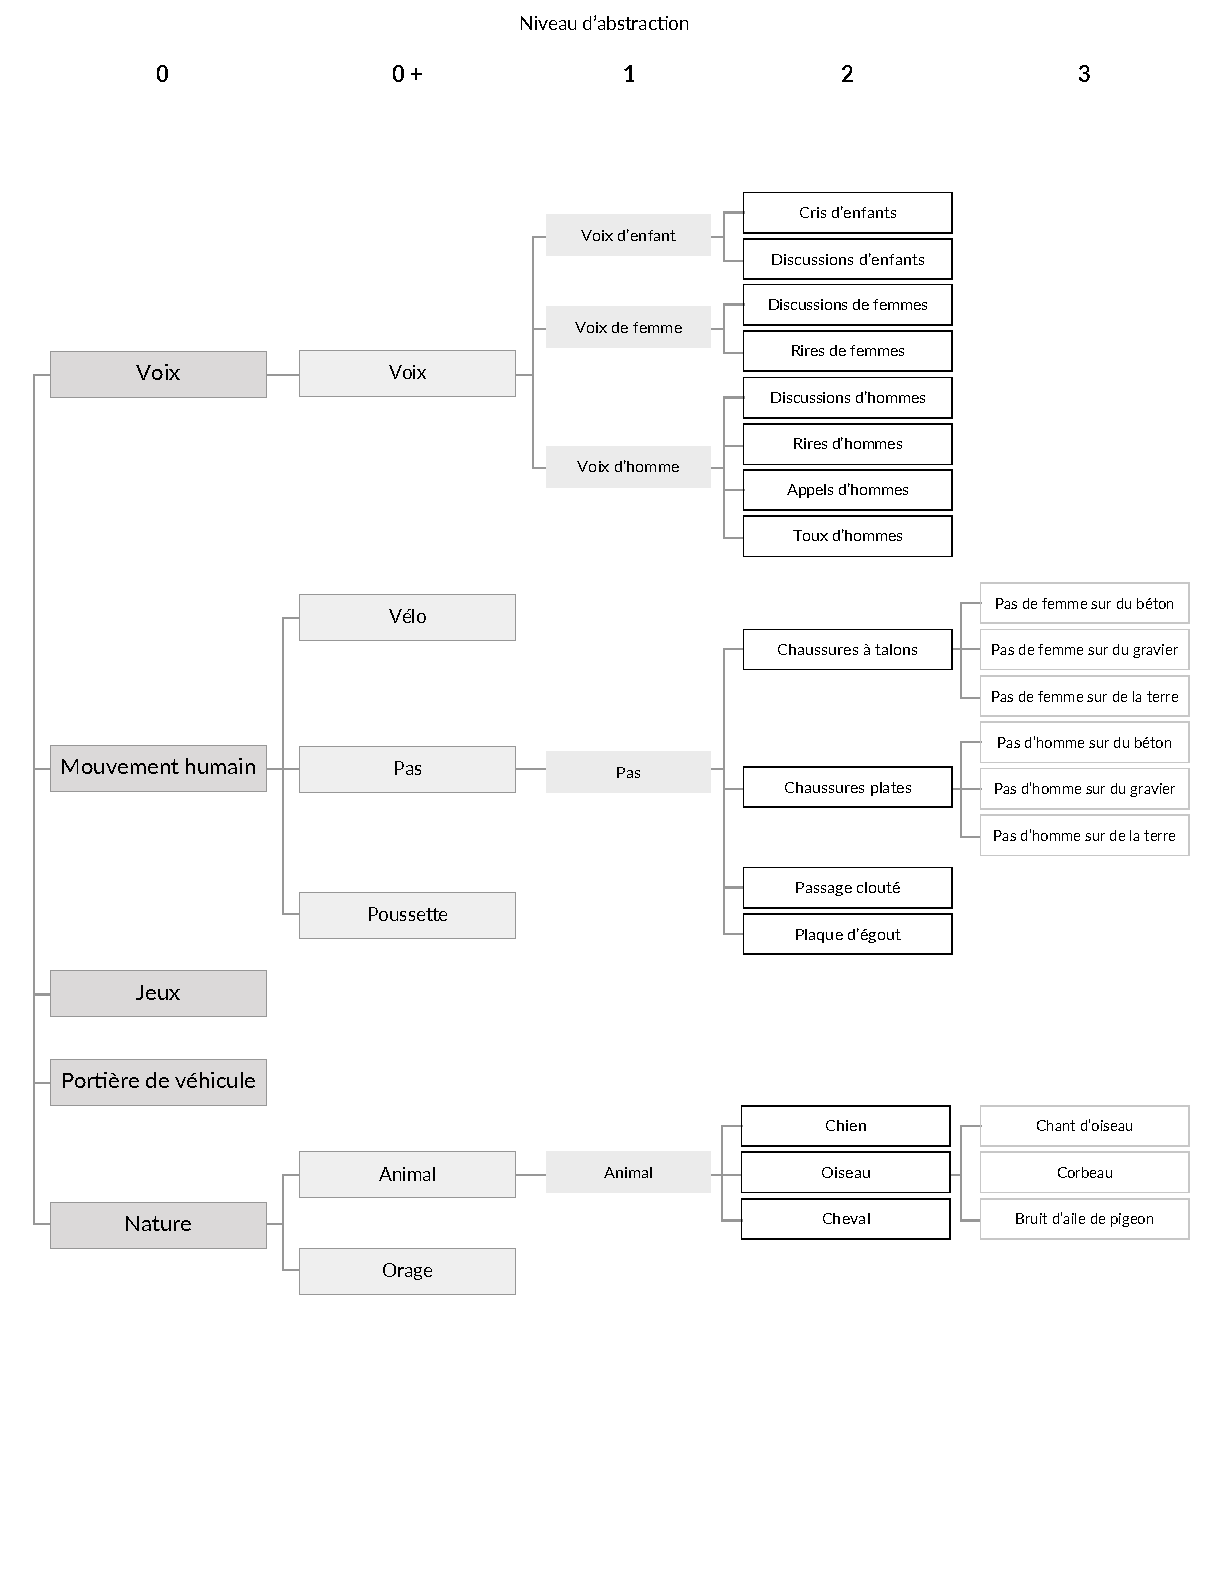
\includegraphics[width=.5\columnwidth]{gfx/ch_5/event_2}\label{fig:taxonomieEventb}}\par
        \subfloat[]
        {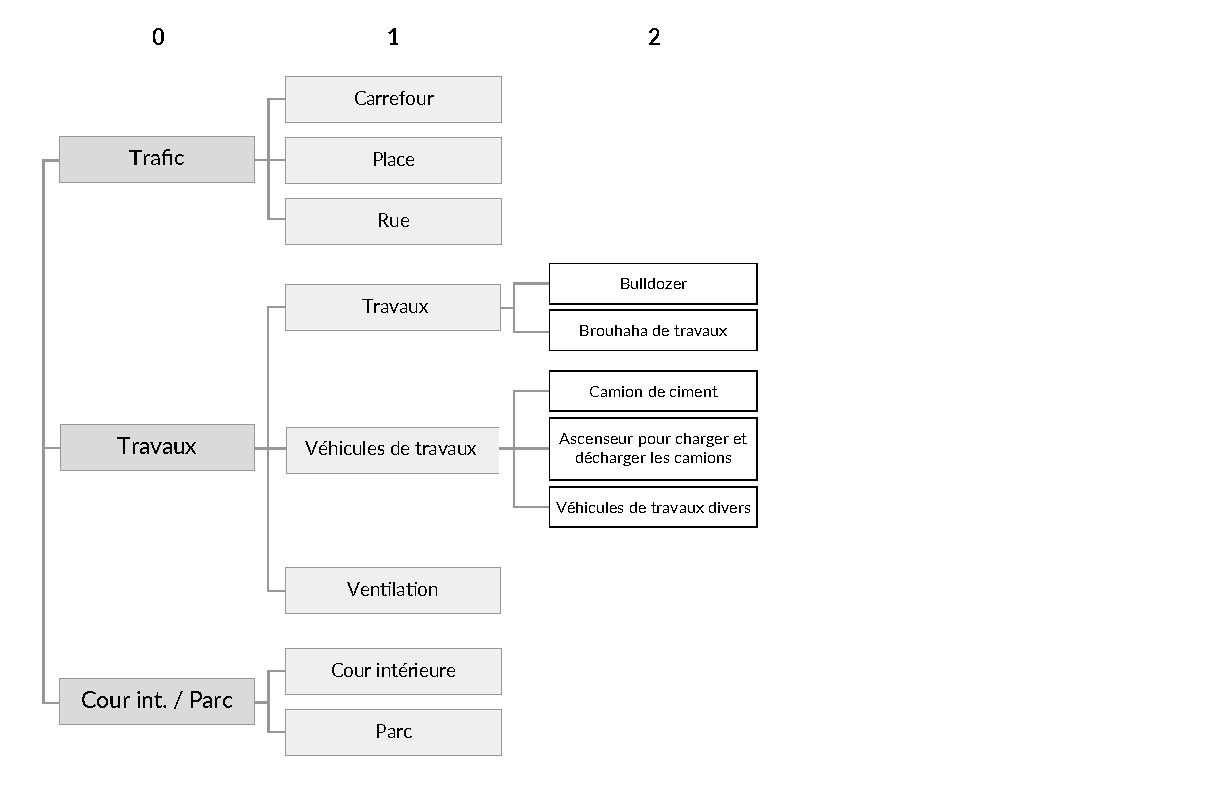
\includegraphics[width=.5\columnwidth]{gfx/ch_5/texture_1}\label{fig:taxonomieTexturea}}
        \subfloat[]
        {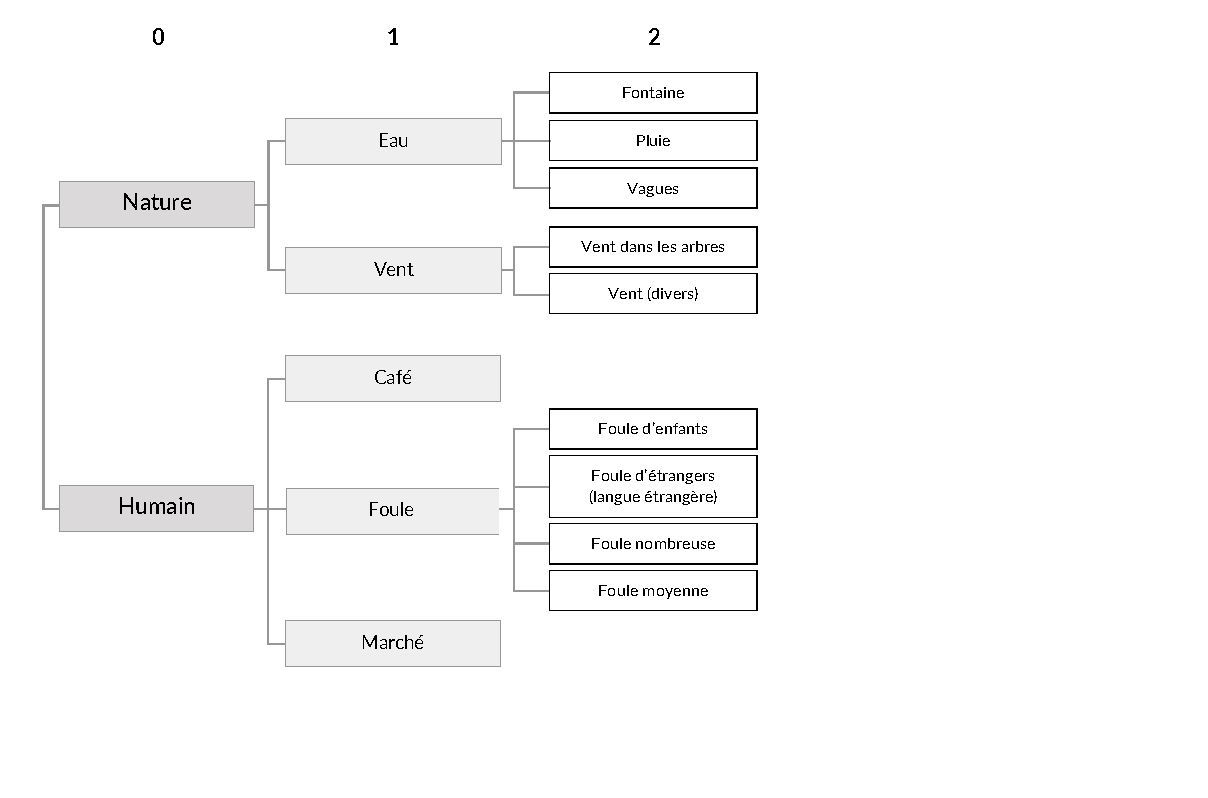
\includegraphics[width=.5\columnwidth]{gfx/ch_5/texture_2}\label{fig:taxonomieTextureb}}
       \caption{Taxonomies des classes de sons utilisées pour la simulation des environnements sonores urbains : (a,b) événements sonores et (c,d) textures sonores.}
       \label{fig:taxonomie}
\end{figure}

\newpage
\section{Dispersions des notes données par les sujets lors de l'expérience 2}
\label{app:xp2}

\begin{figure}[h]
        \myfloatalign
        \subfloat[sujet 1]
        {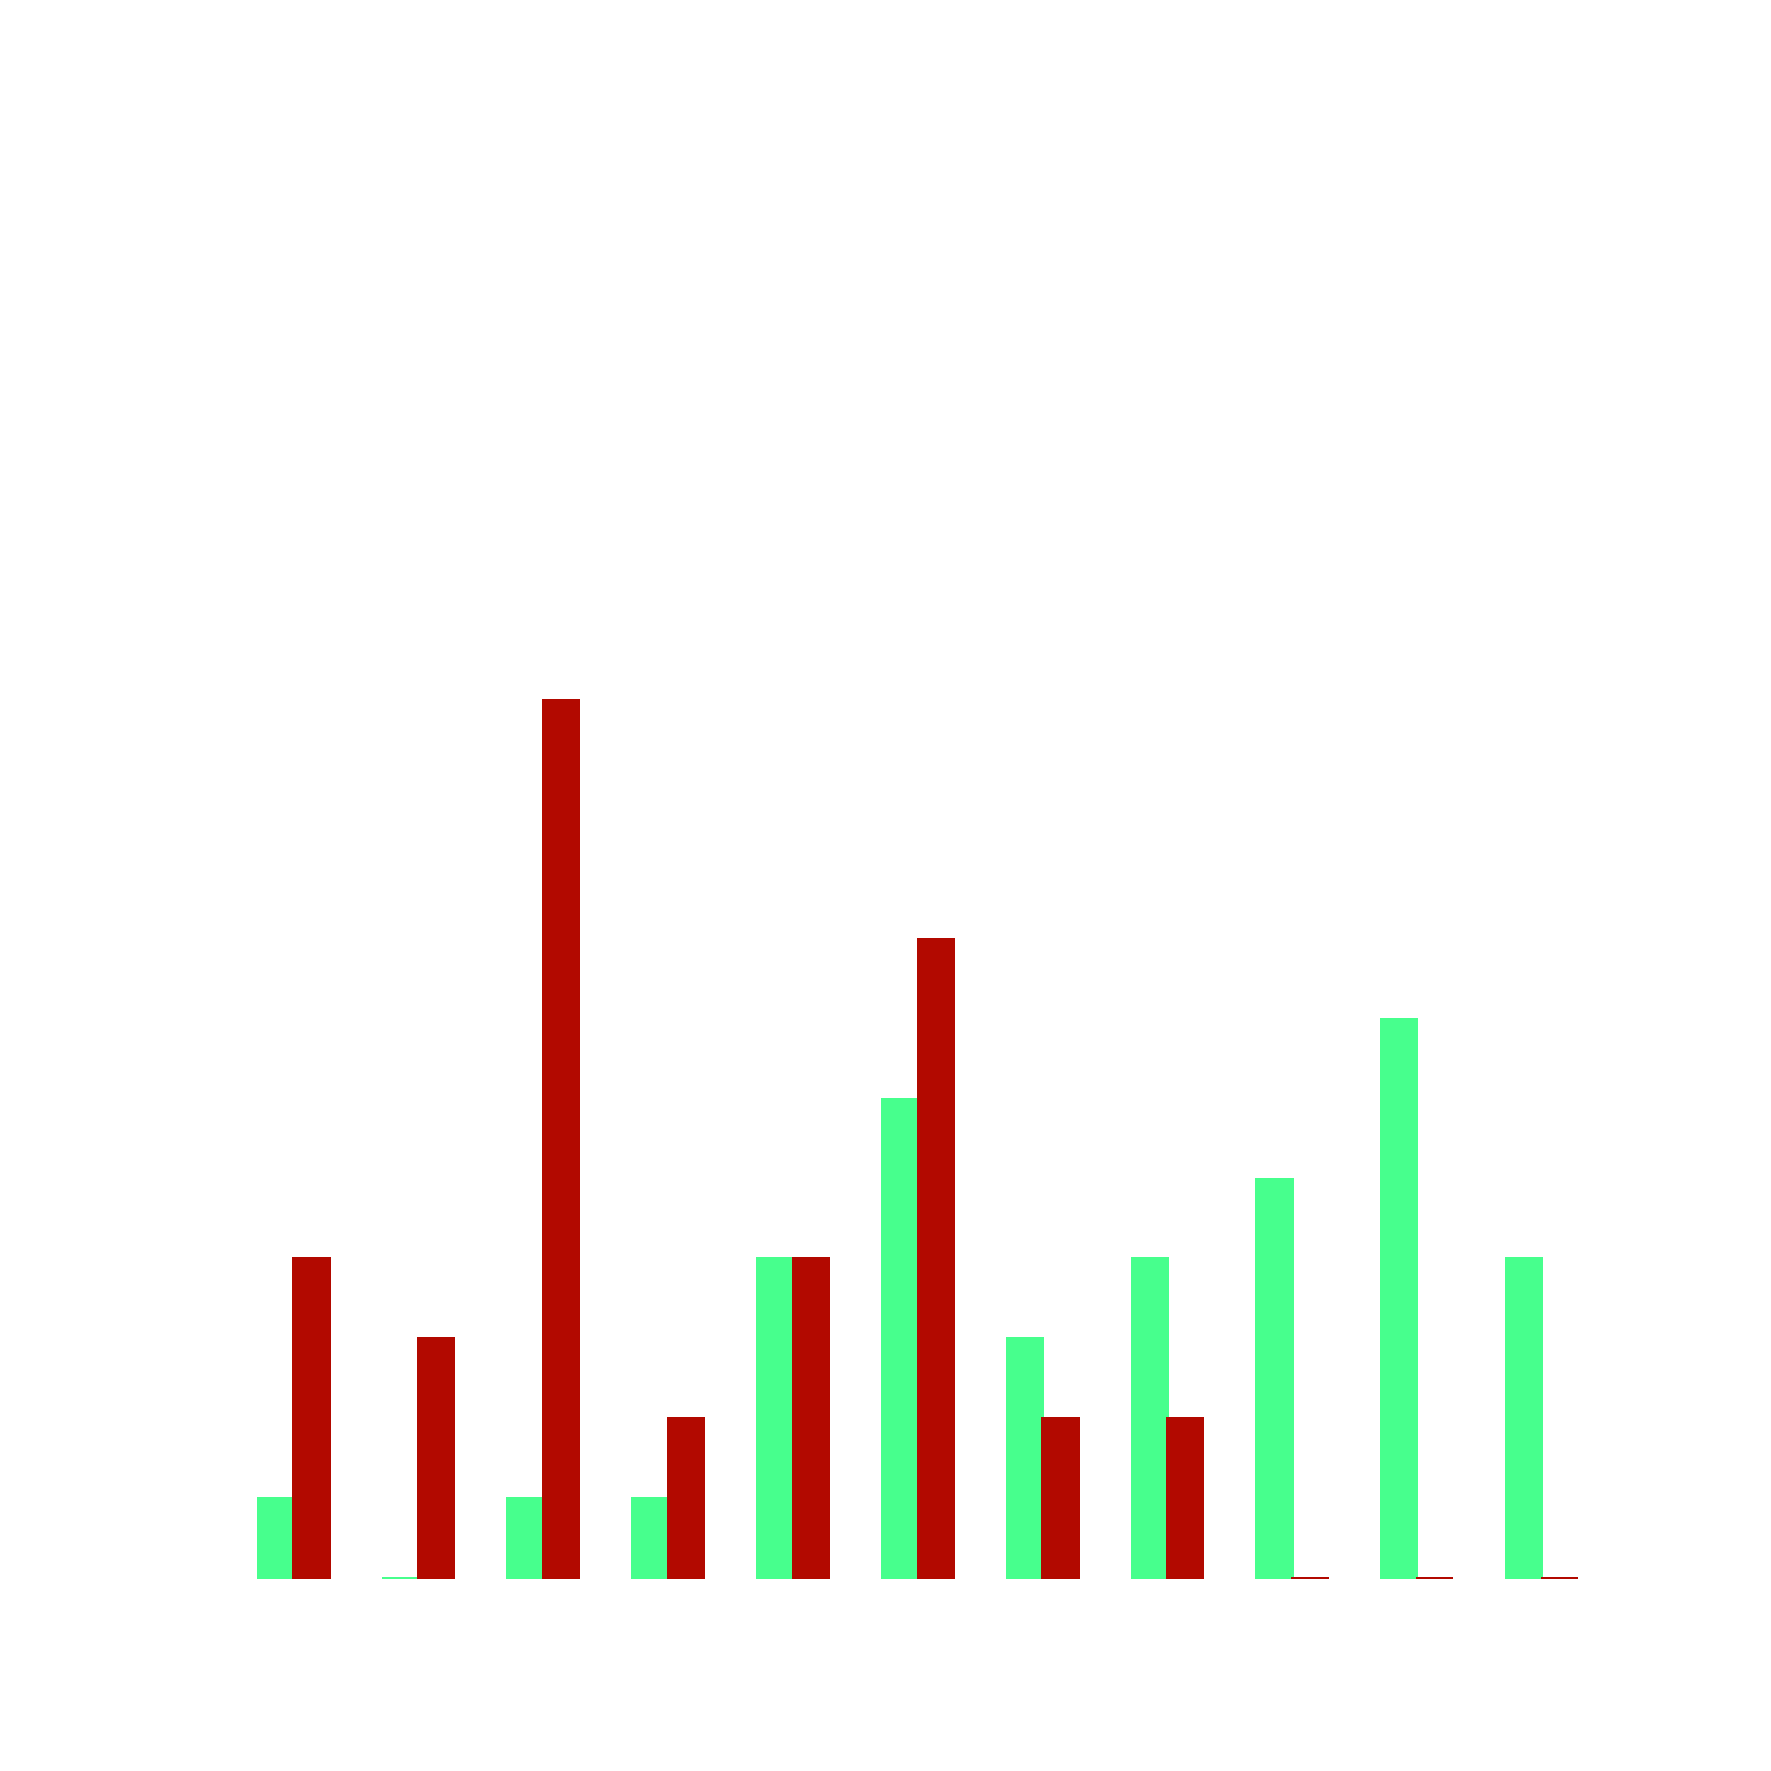
\includegraphics[width=.24\linewidth]{gfx/ch_5/xp4_note_1}\label{fig:xp4_note_1a}}
        \subfloat[sujet 2]
        {\includegraphics[width=.24\linewidth]{gfx/ch_5/xp4_note_2}\label{fig:xp4_note_1b}}
        \subfloat[sujet 3]
        {\includegraphics[width=.24\linewidth]{gfx/ch_5/xp4_note_3}\label{fig:xp4_note_1c}}
        \subfloat[sujet 4]
        {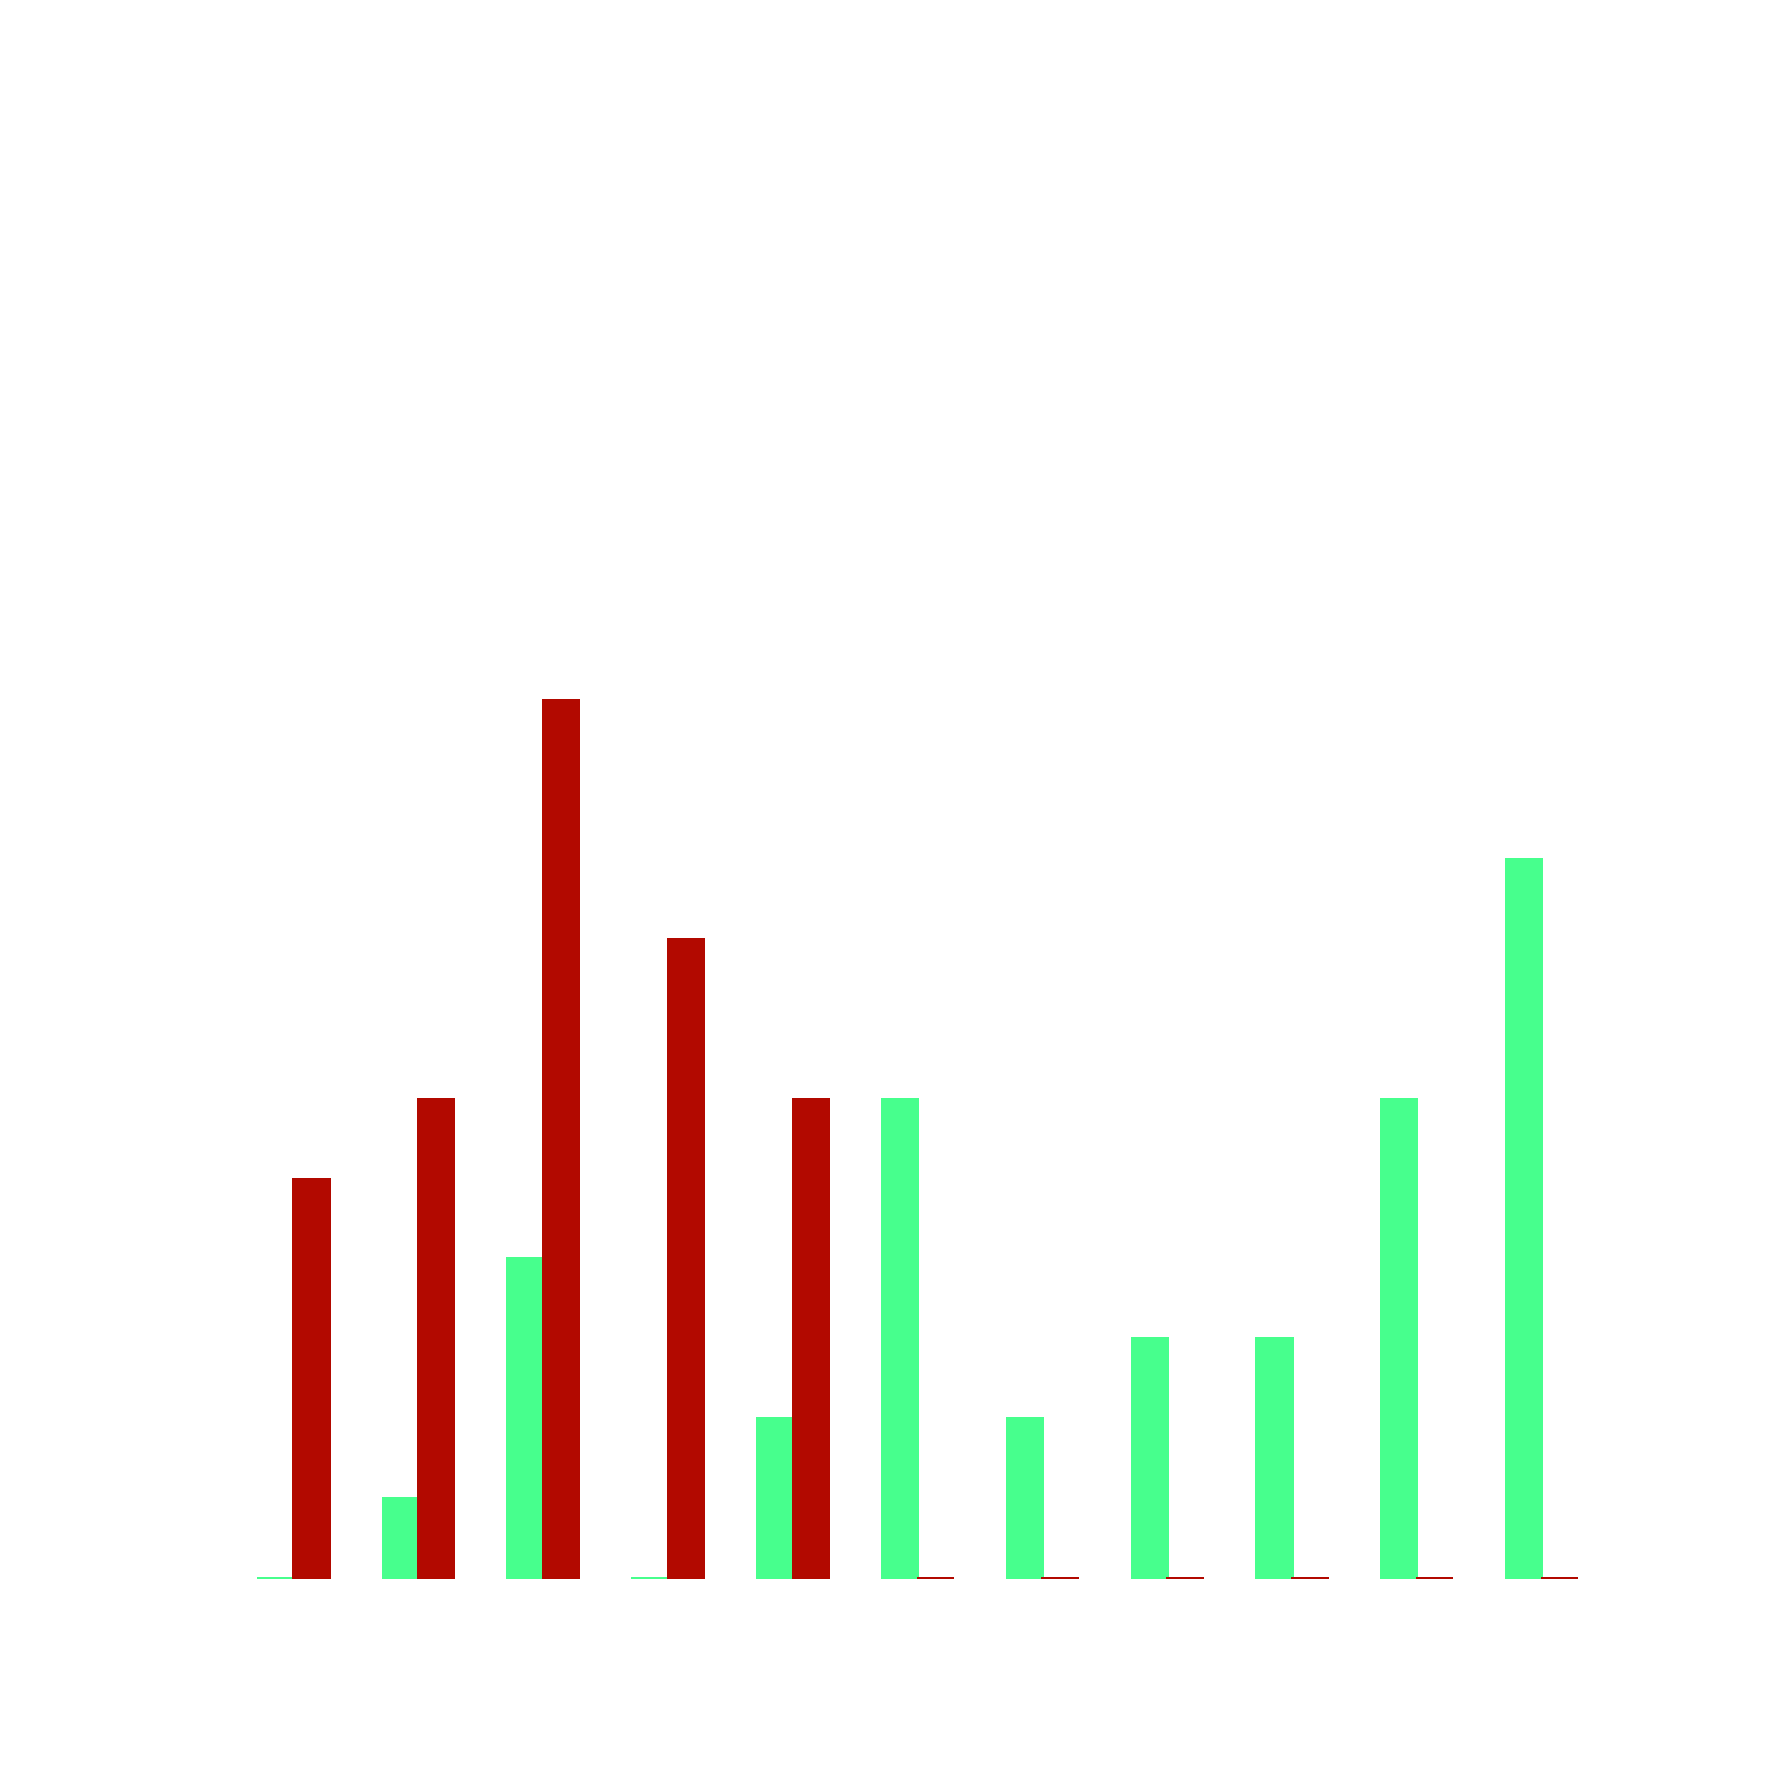
\includegraphics[width=.24\linewidth]{gfx/ch_5/xp4_note_4}\label{fig:xp4_note_1d}} \par
        \subfloat[sujet 5]
        {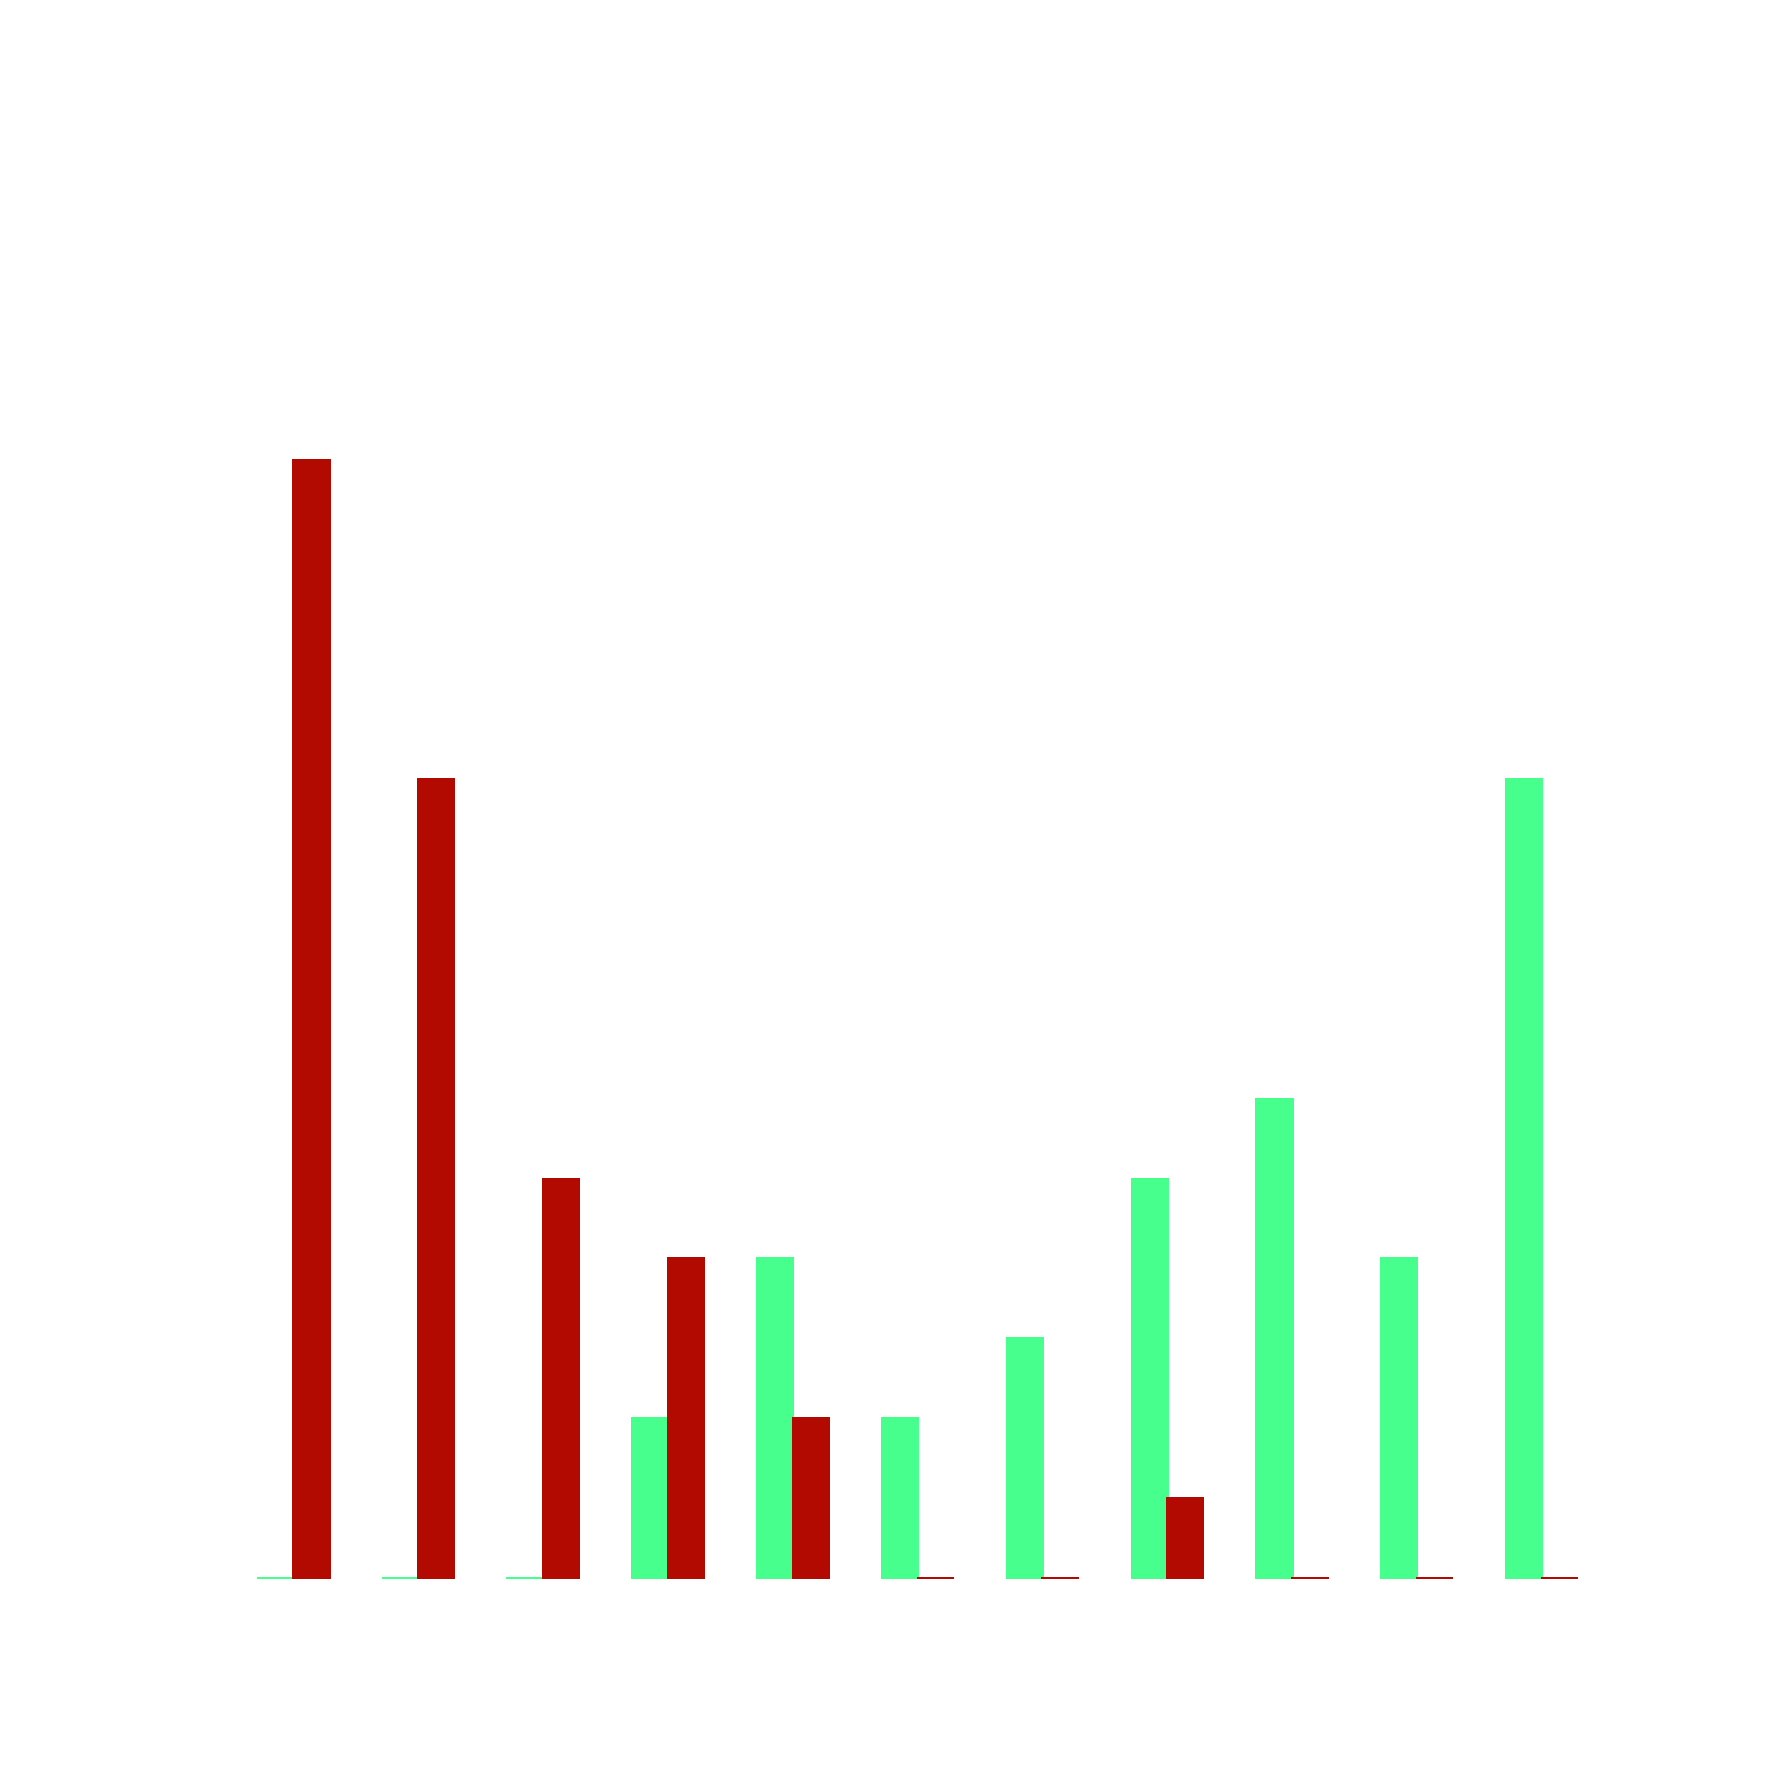
\includegraphics[width=.24\linewidth]{gfx/ch_5/xp4_note_5}\label{fig:xp4_note_1e}}
        \subfloat[sujet 6]
        {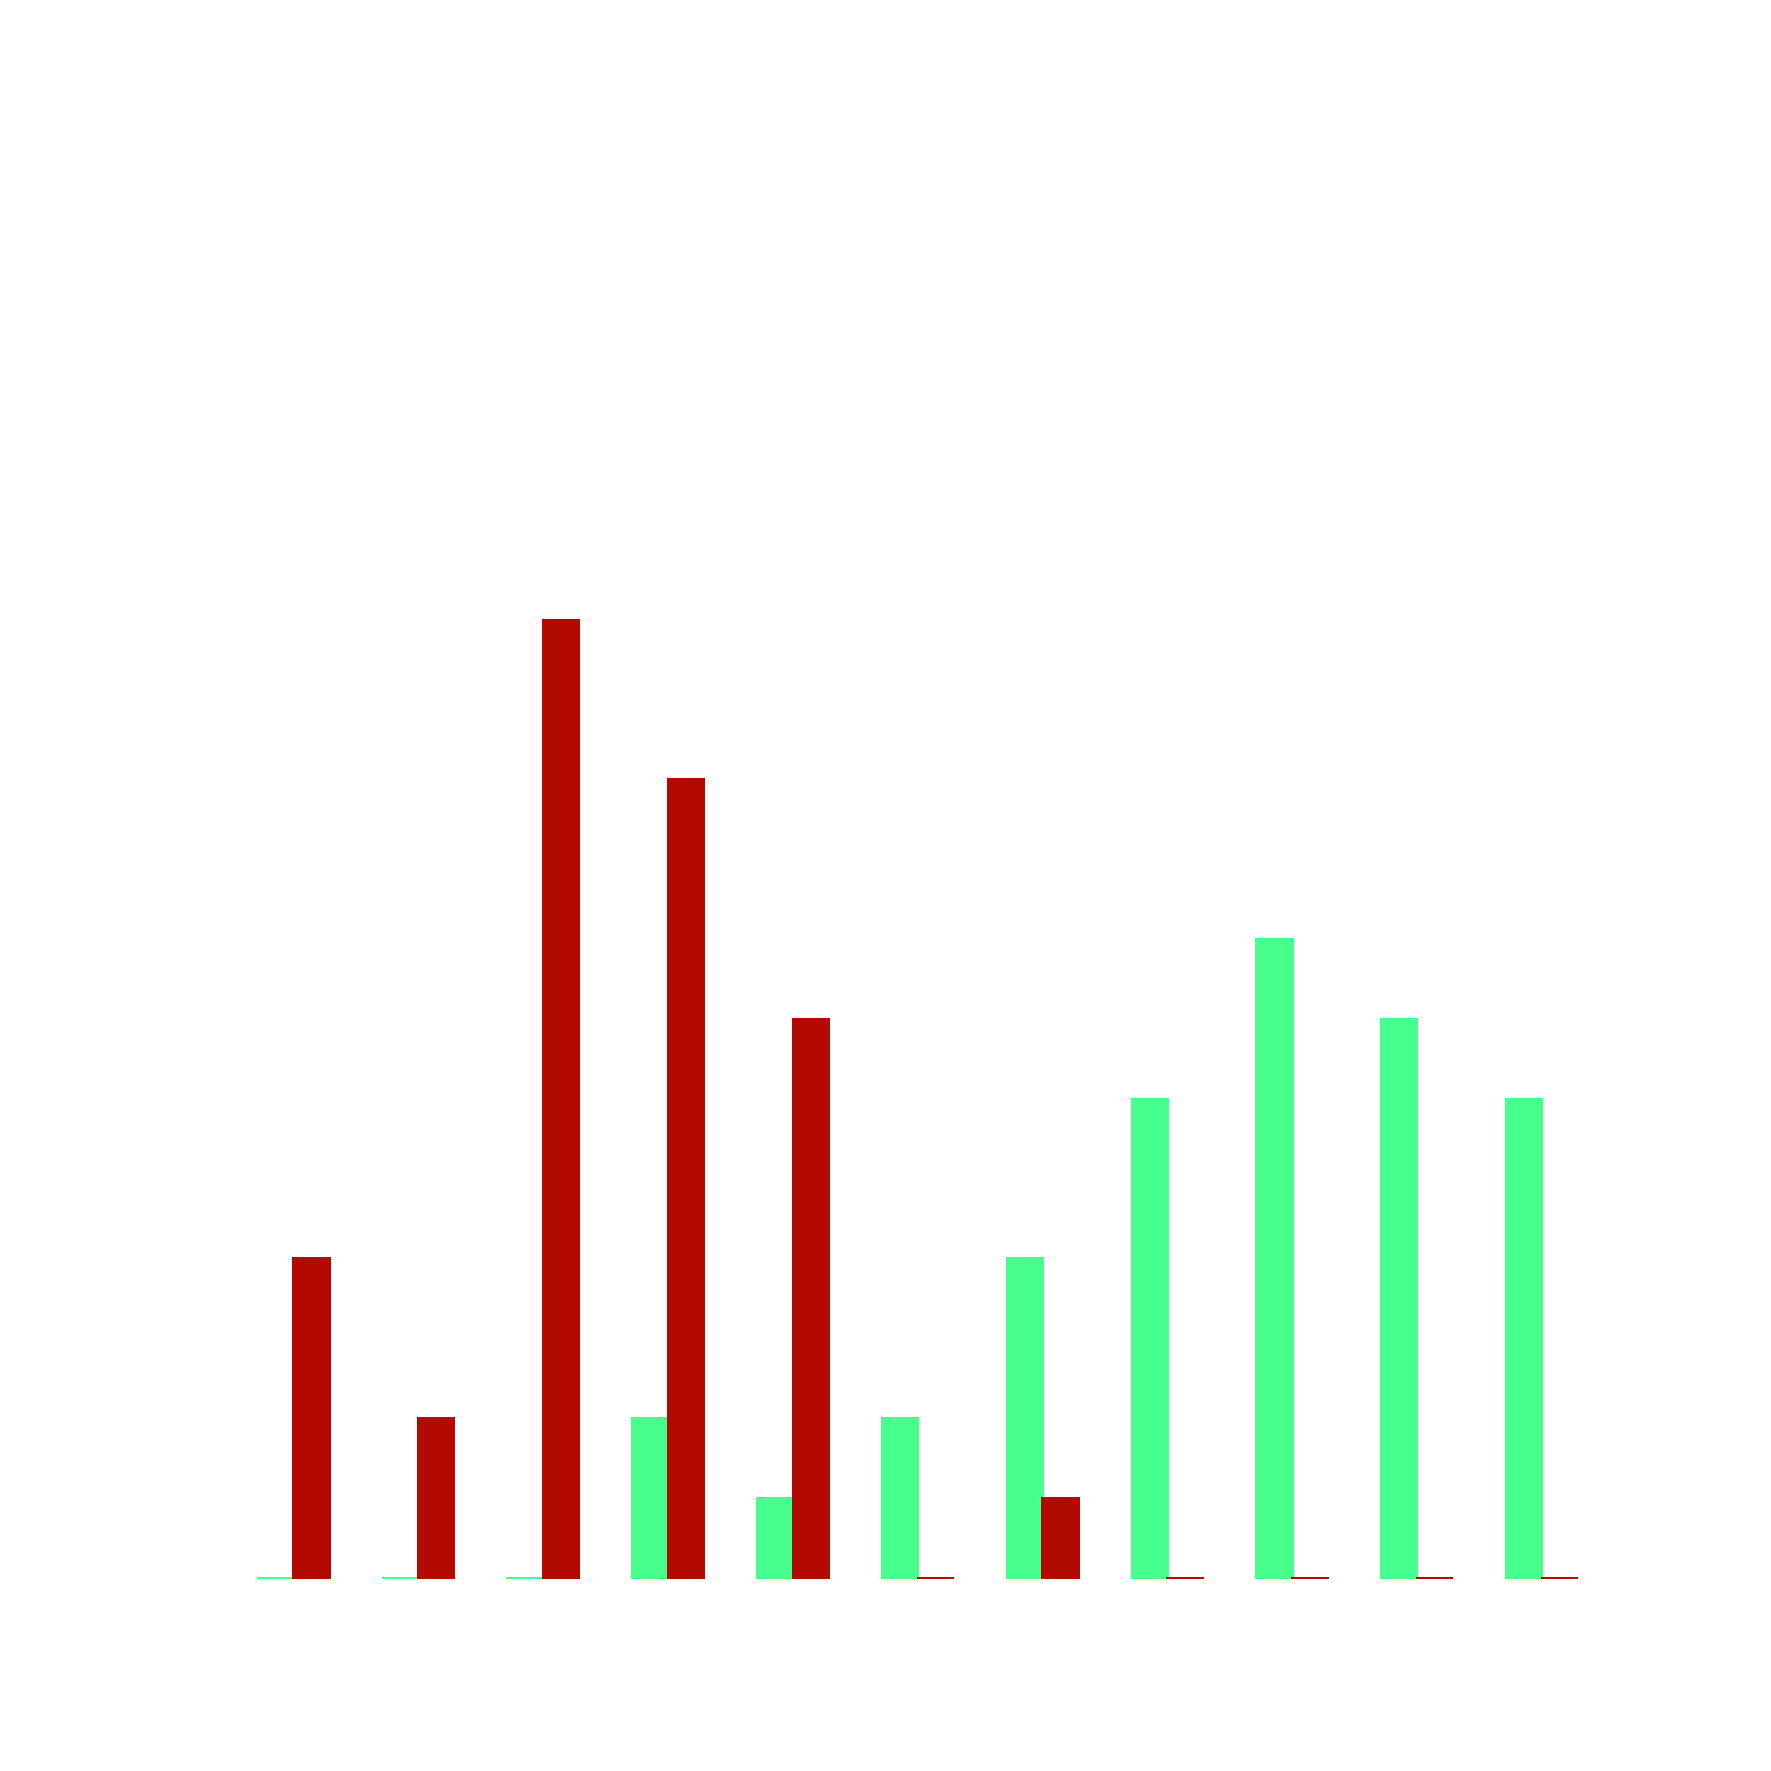
\includegraphics[width=.24\linewidth]{gfx/ch_5/xp4_note_6}\label{fig:xp4_note_1f}}
        \subfloat[sujet 7]
        {\includegraphics[width=.24\linewidth]{gfx/ch_5/xp4_note_7}\label{fig:xp4_note_1g}}
        \subfloat[sujet 8]
        {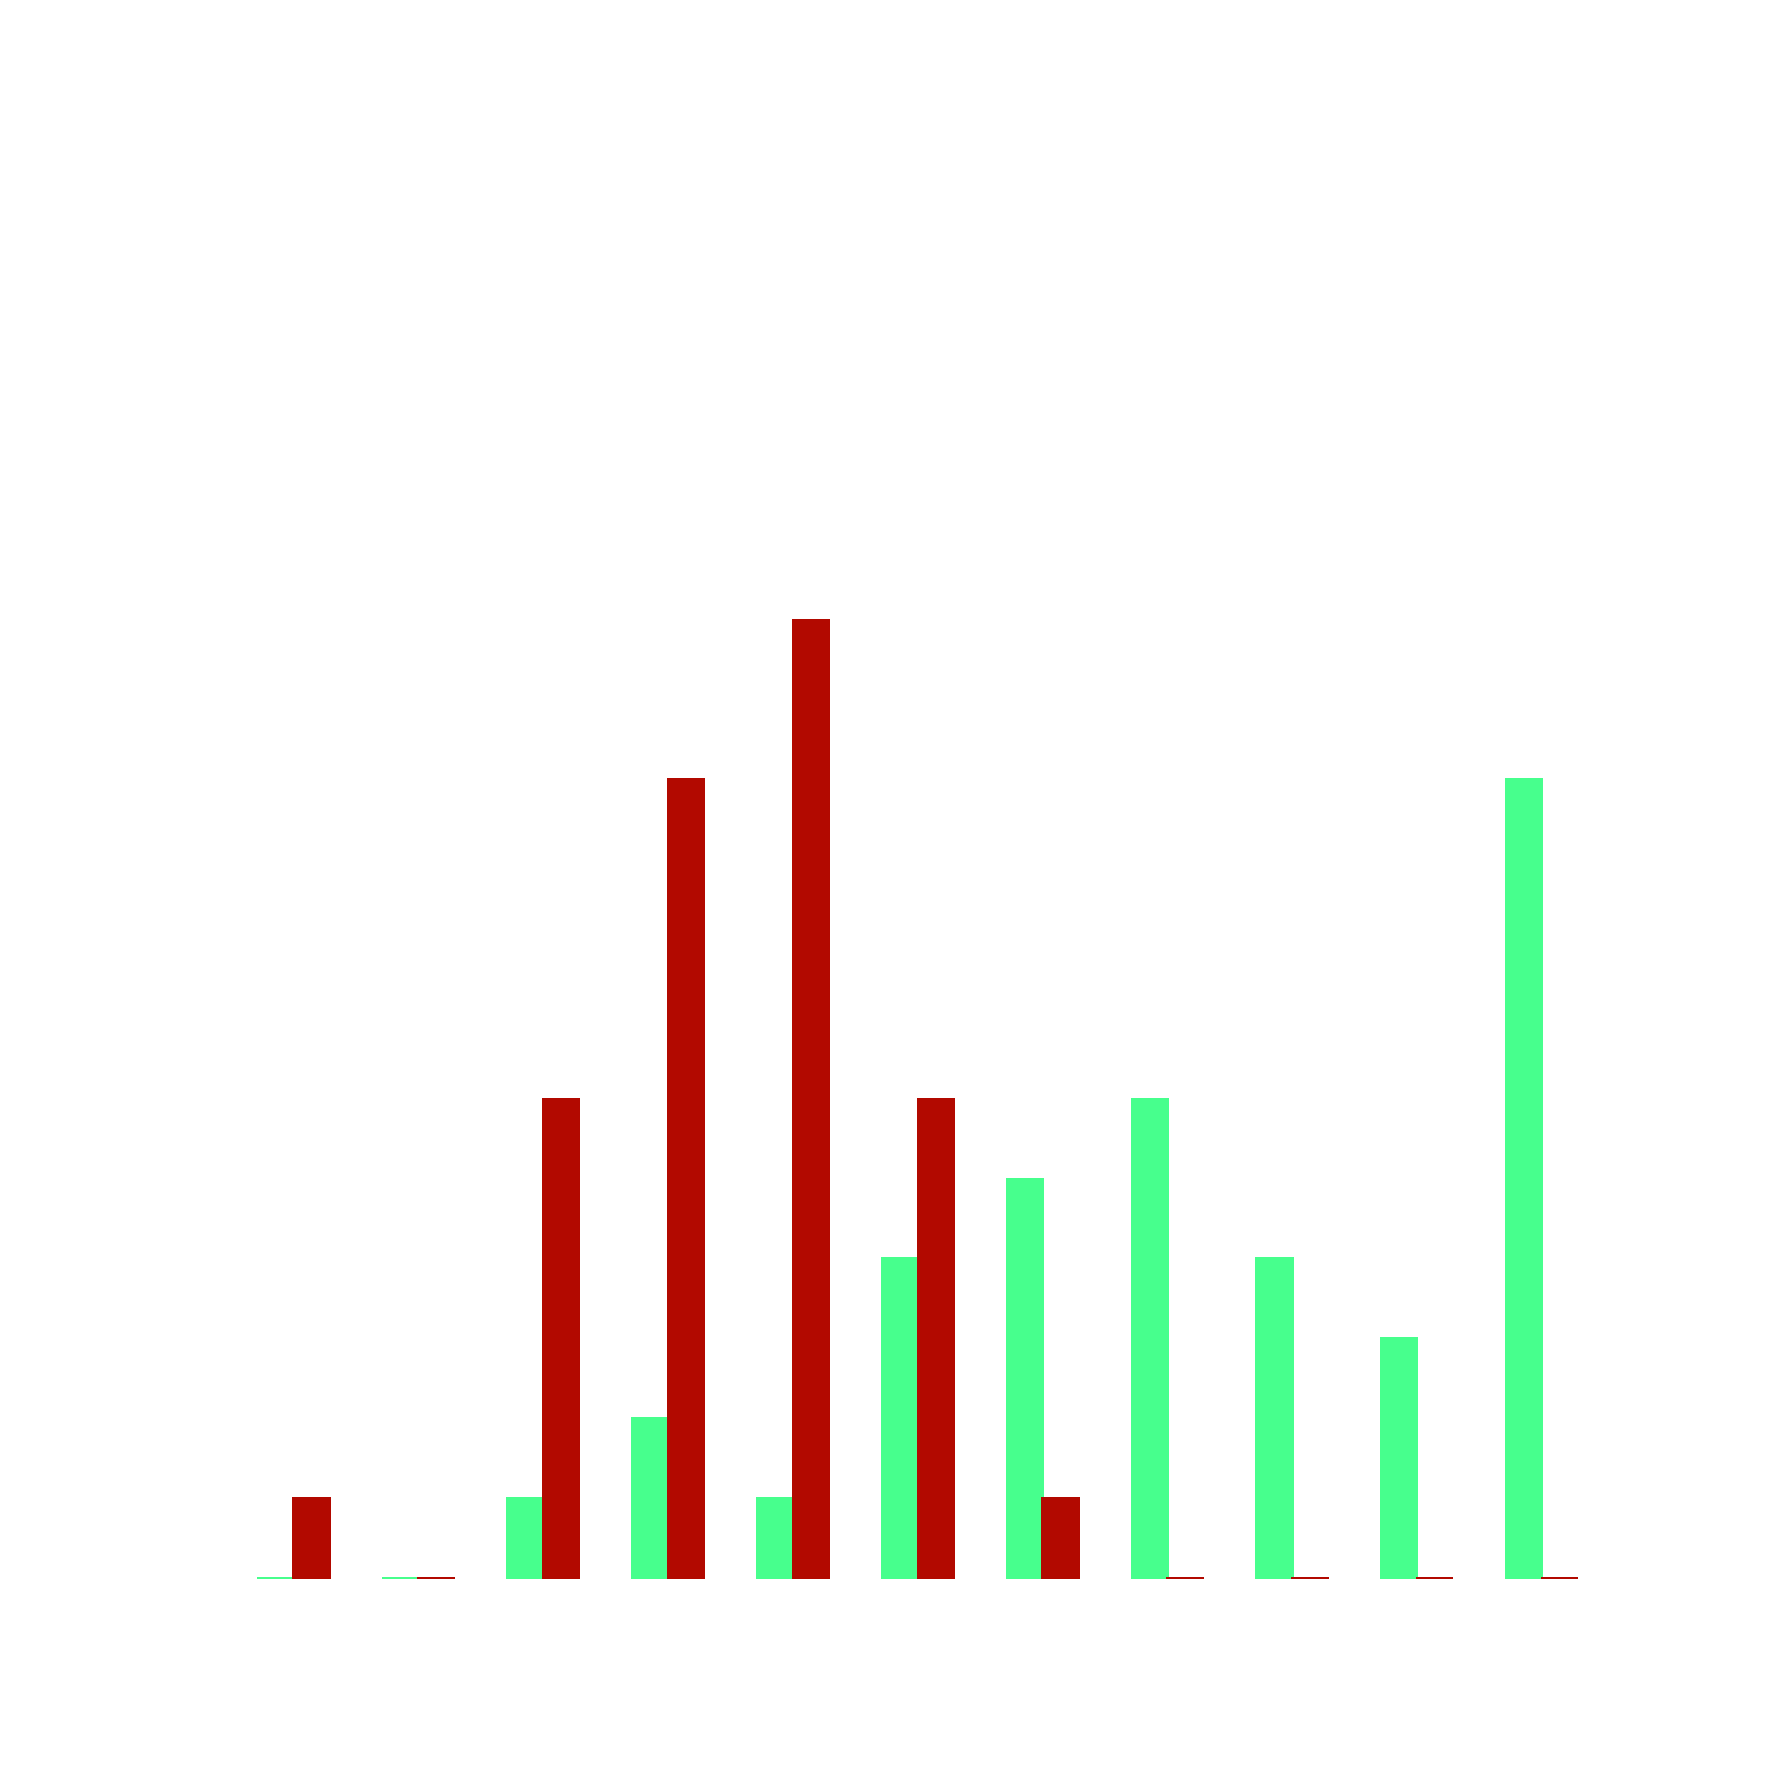
\includegraphics[width=.24\linewidth]{gfx/ch_5/xp4_note_8}\label{}} \par
        \subfloat[sujet 9]
        {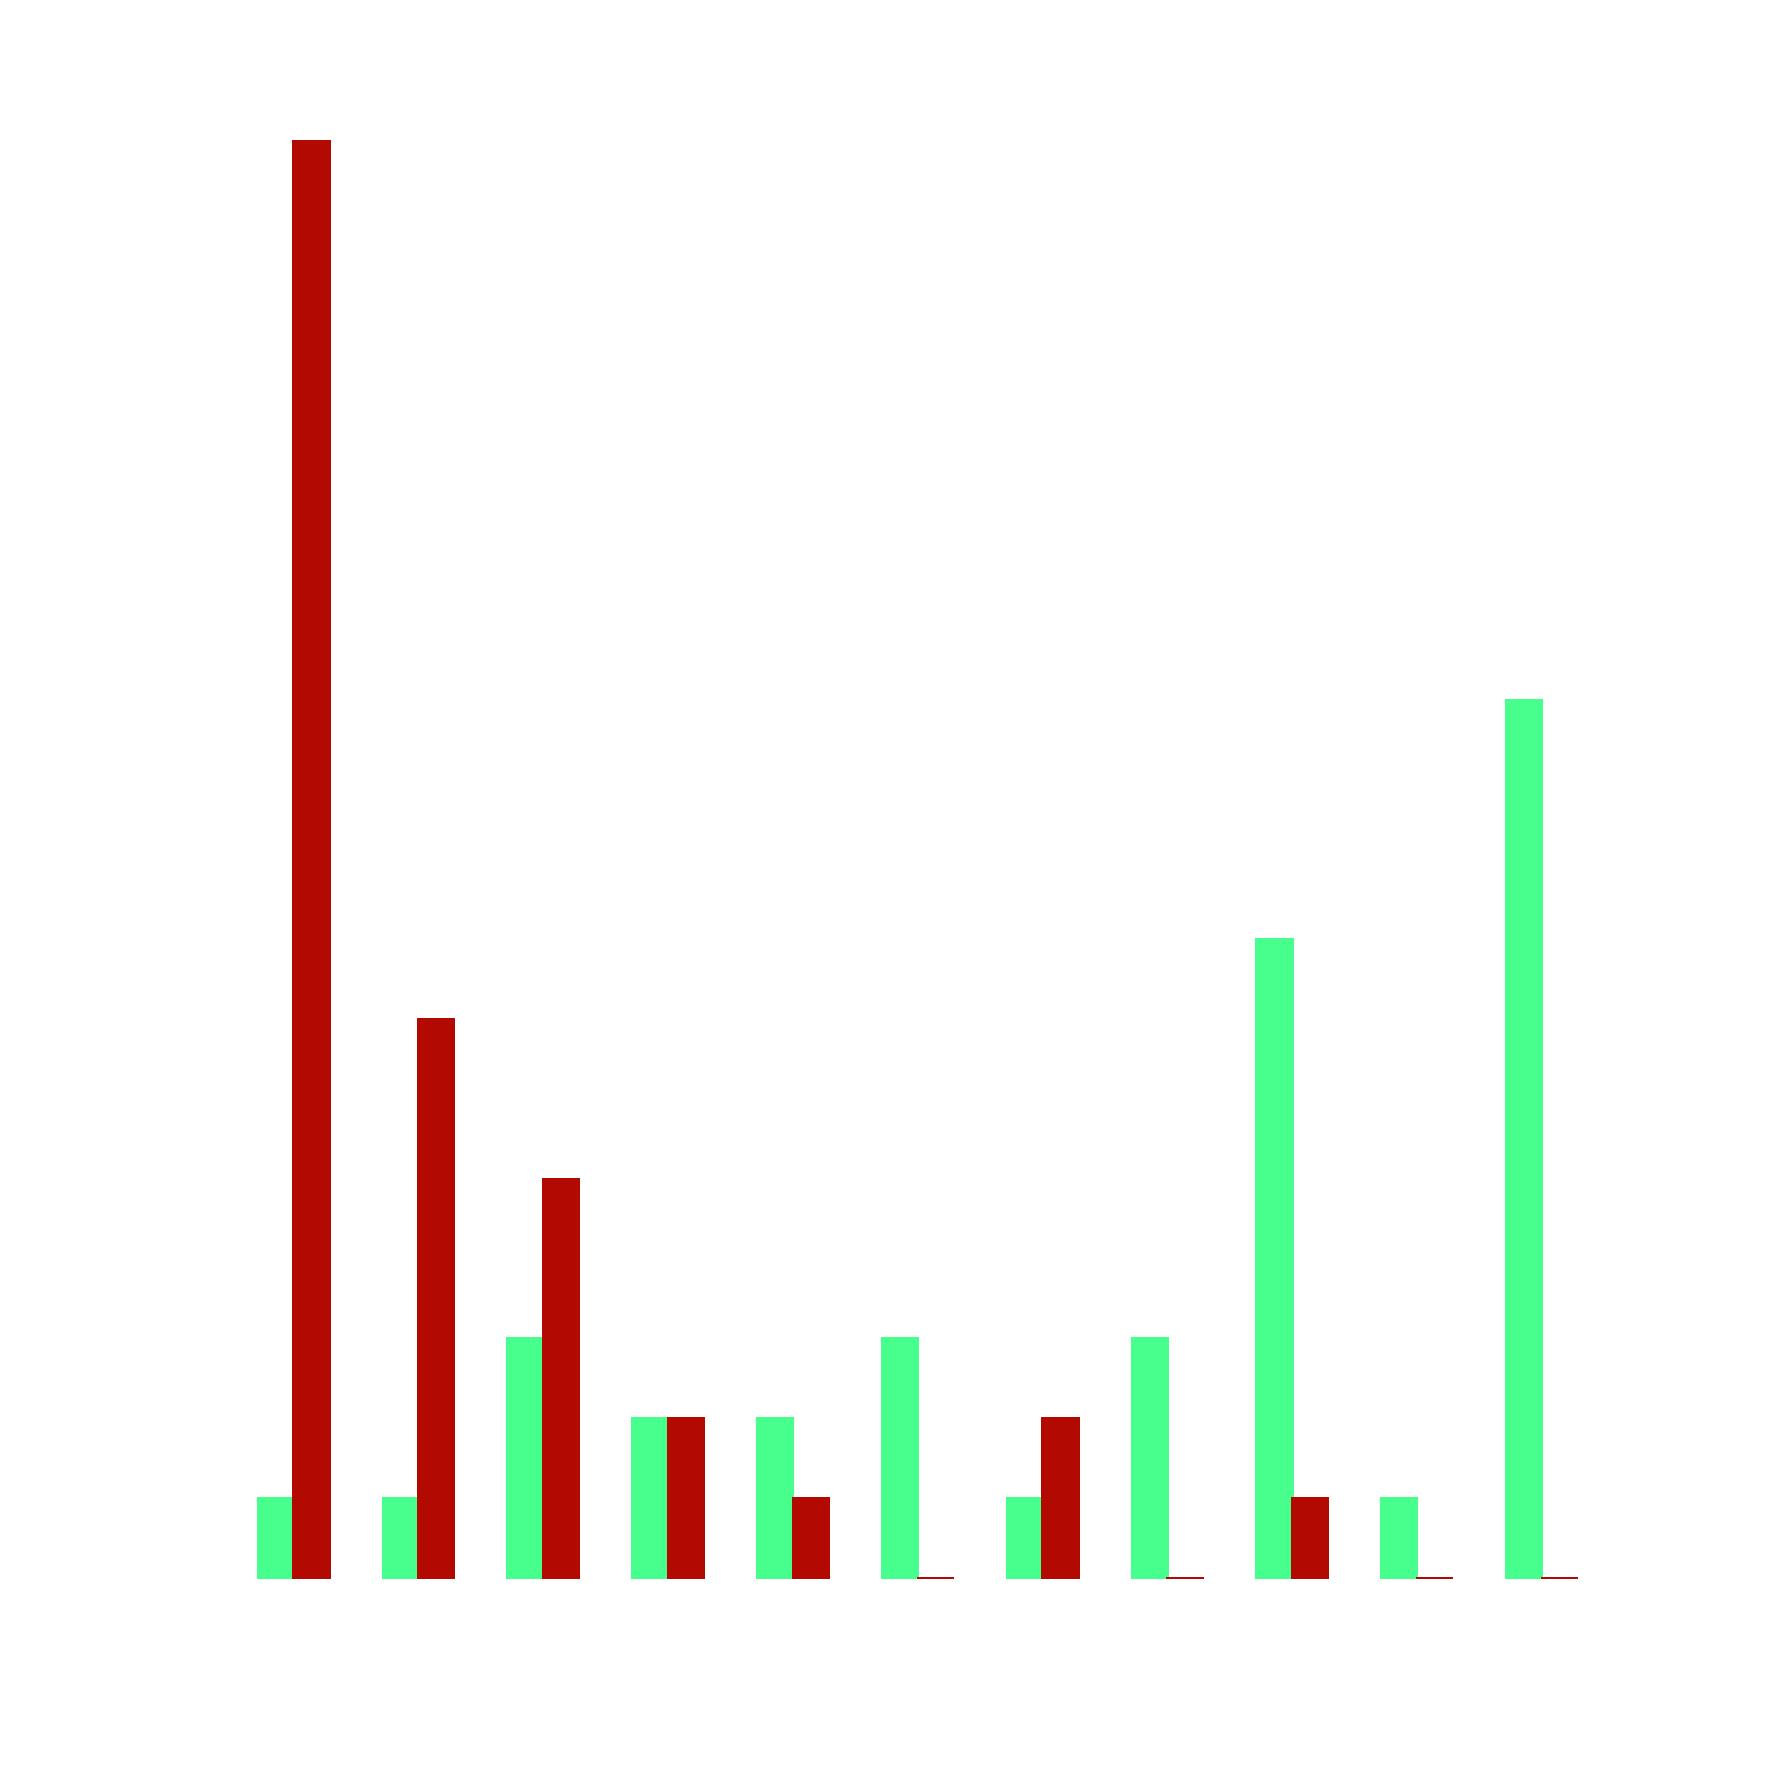
\includegraphics[width=.24\linewidth]{gfx/ch_5/xp4_note_9}\label{fig:xp4_note_1i}}
        \subfloat[sujet 10]
        {\includegraphics[width=.24\linewidth]{gfx/ch_5/xp4_note_10}\label{fig:xp4_note_1j}}
        \subfloat[sujet 11]
        {\includegraphics[width=.24\linewidth]{gfx/ch_5/xp4_note_11}\label{fig:xp4_note_1z}}
        \subfloat[sujet 12]
        {\includegraphics[width=.24\linewidth]{gfx/ch_5/xp4_note_12}\label{fig:xp4_note_1l}}
        \caption{Dispersions des notes données par les sujets lors de l'expérience 2 aux i/am-scènes (vert) et ni/am-scènes (rouge).}\label{fig:xp4_note_1}
\end{figure}

\end{document}
